%!TEX TS-program = pdflatex
%!TEX encoding = UTF-8 Unicode

\documentclass[12pt,a4paper,twoside,english,italian]{book}
\usepackage[utf8]{inputenc}
\usepackage[italian]{babel}
\usepackage[T1]{fontenc}
\usepackage{listings}
\usepackage{hyperref}
\usepackage{enumerate}
\usepackage{pdfpages}
\usepackage{afterpage}
\usepackage{xcolor}
\usepackage{sectsty}
\usepackage{color}
\usepackage{uniudtesi}

\makeatletter
\newcommand\BeraMonottfamily{%
	\def\fvm@Scale{0.85}% scales the font down
	\fontfamily{fvm}\selectfont% selects the Bera Mono font
}
\makeatother

\definecolor{gray}{rgb}{0.4,0.4,0.4}
\definecolor{darkblue}{rgb}{0.0,0.0,0.6}
\definecolor{cyan}{rgb}{0.0,0.6,0.6}
\definecolor{maroon}{rgb}{0.5,0,0}
\definecolor{darkgreen}{rgb}{0,0.5,0}

\lstset{
	basicstyle=\ttfamily,
	columns=fullflexible,
	showstringspaces=false,
	commentstyle=\color{gray}\upshape,
	aboveskip=20pt,
	belowskip=20pt,
	breaklines=true,
}

\lstdefinelanguage{XML}
{
	basicstyle=\ttfamily,
	morestring=[s]{"}{"},
	morecomment=[s]{?}{?},
	morecomment=[s]{!--}{--},
	commentstyle=\color{darkgreen},
	moredelim=[s][\color{black}]{>}{<},
	moredelim=[s][\color{red}]{\ }{=},
	stringstyle=\color{blue},
	identifierstyle=\color{maroon},
	breaklines=true,
	postbreak=\mbox{\textcolor{red}{$\hookrightarrow$}\space},
	captionpos=b,
	frame=tb,
}

% Col pacchetto tocbibind compariranno nell'indice anche
% la bibliografia ed eventualmente l'indice analitico
\usepackage[nottoc]{tocbibind}

% Il pacchetto indentfirst abolisce la fastidiosa convenzione
% anglosassone di fa cominciare la prima riga di un
% capitolo o sezione a margine sinistro, senza rientro:
\usepackage{indentfirst}

% \usepackage{graphicx} % gia' caricato da uniudtesi
\graphicspath{{./figure/}}

\usepackage{amsmath,amsfonts,amssymb,amsthm}
\usepackage{latexsym}

\newcommand{\N}{\mathbb{N}}
\newcommand{\Z}{\mathbb{Z}}
\newcommand{\Q}{\mathbb{Q}}
\newcommand{\R}{\mathbb{R}}
\newcommand{\C}{\mathbb{C}}

\DeclareMathOperator{\traccia}{tr}
\DeclareMathOperator{\sen}{sen}
\DeclareMathOperator{\arcsen}{arcsen}
\DeclareMathOperator*{\maxlim}{max\,lim}
\DeclareMathOperator*{\minlim}{min\,lim}
\DeclareMathOperator*{\deepinf}{\phantom{\makebox[0pt]{p}}inf}

\newcommand{\varsum}[3]{\sum_{#2}^{#3}\!
	{\vphantom{\sum}}_{#1}\;}
\newcommand{\varprod}[3]{\sum_{#2}^{#3}\!
	{\vphantom{\sum}}_{#1}\;}


\theoremstyle{plain}
\newtheorem{teorema}{Teorema}[chapter]
\newtheorem{proposizione}[teorema]{Proposizione}
\newtheorem{lemma}[teorema]{Lemma}
\newtheorem{corollario}[teorema]{Corollario}

\theoremstyle{definition}
\newtheorem{definizione}[teorema]{Definizione}
\newtheorem{esempio}[teorema]{Esempio}

\theoremstyle{remark}
\newtheorem{osservazione}[teorema]{Osservazione}

\usepackage{fancyhdr}
\pagestyle{fancy}
\fancyhf{}
\fancyhead[LE,RO]{\bfseries\thepage}
\fancyhead[LO]{\bfseries\rightmark}
\fancyhead[RE]{\bfseries\leftmark}
\renewcommand{\headrulewidth}{0.5pt}
\renewcommand{\footrulewidth}{0pt}
\setlength{\headheight}{14.5pt}

\begin{document}
\frontmatter
%\maketitle
\begin{titlepage}
	\begin{sffamily}
		\begin{large}
			\begin{center}
				\vbox to0pt{%
					\vbox to\textheight{\vfil
						
\includegraphics[width=\textwidth]{polloPallido}%
						\vfil}\vss}
			\end{center}
			\begin{center}
				\begin{Large}
					\uppercase{Universit\`a degli Studi di Udine}
				\end{Large}\\
				\rule{9cm}{.4pt}\\
				\smallskip
				 Dipartimento di Scienze Matematiche, Informatiche e Fisiche\\
				\medskip
				\rule{9cm}{.4pt}\\
				Corso di Sistemi Distribuiti\\
				\bigskip\vfill
				\bigskip
				\bigskip
				{\vfil
					\begin{Huge}
					Relazione del progetto 
					\end{Huge}%
					\begin{LARGE}

							
					\end{LARGE}}
				\bigskip\vfill
				\end{center}
			\begin{center}
				\vfill
				\rule{9cm}{.4pt}\\
				\bigskip
				\uppercase{Docente}: Marino Miculan\\
				\medskip
				\uppercase{Studente}: Andreussi Angelo\\
				\uppercase{Studente}: Forgiarini Alessandro\\
			\end{center}
			\begin{center}
				\vfill
				\rule{9cm}{.4pt}\\
				\medskip
				\uppercase{Anno Accademico 2019 - 2020}\\
			\end{center}
		\end{large}
	\end{sffamily}
	\clearemptydoublepage
\end{titlepage}



\renewcommand{\theequation}{\arabic{equation}}%consigliato per migliorare i numeri di equazione nell'introduzione
\renewcommand{\thesection}{\arabic{section}}%consigliato per migliorare i numeri di equazione nell'introduzione

%!TEX TS-program = pdflatex
%!TEX root = progetto_finale.tex
%!TEX encoding = UTF-8 Unicode

\chapter{Introduzione}

Il problema in esame consiste nella gestione dei taxi elettrici e assegnazione di essi agli utenti che ne fanno richiesta per spostarsi all'interno di una città. Si vuole creare un sistema distribuito in modo che non sia necessario un server centralizzato, in tal modo sono le vetture che si accordano tra di loro, attraverso un meccanismo di comunicazione wireless, per decidere la migliore vettura che possa soddisfare la richiesta del cliente. Allo stesso modo, il cliente richiede il servizio comunicando direttamente con una di queste macchine, con lo stesso metodo di comunicazione senza fili. 

La soluzione proposta consiste in:
\begin{enumerate}
	\item L'utente invia la richiesta di spostamento al taxi a lui più vicino indicando la propria posizione e destinazione.
	\item La vettura riceve la richiesta e, comunicando con gli altri taxi, viene deciso quale veicolo è il più adatto per soddisfare il bisogno dell'utente.
	\item Per decidere quale sia la vettura più adatta, si prendono in considerazione diversi parametri, tra cui: distanza dall'utente, carica rimanente e se la vettura al momento è già occupata.
	\item Notifica al cliente da parte della macchina di essere stata scelta per il trasporto.
	\item Il veicolo scelto si sposta verso l'utente e lo trasporta verso la direzione richiesta.
\end{enumerate}

\section{Problemi del sistema distribuito} \label{problematiche_distribuite}

Alcuni problemi che potrebbero emergere in questo contesto, interessanti da affrontare nella costruzione del sistema distribuito, sono la possibilità di rottura di un veicolo, il cambio destinazione di un utente, la rottura di una strada della città.

Si potrebbe pensare che nella realtà, a seguito dell'inagibilità di una strada, una parte della città sia isolata dal resto. Questa situazione non viene presa in considerazione, infatti in uno scenario reale la disconnessione della città è praticamente impossibile poiché vi sono strade alternative che garantiscono un percorso.

Si potrebbe anche pensare che un veicolo, a seguito di uno spostamento, si isoli e non sia più in grado di comunicare con le altre vetture. Questa situazione è realistica, tuttavia non è problematica visto che gli algoritmi utilizzati non prevedono una connessione completa del grafo di comunicazione delle macchine.

I clienti che richiedono il servizio inoltrano la propria richiesta a delle speciali celle riservate alla comunicazione cliente-taxi, simili a dei ripetitori, che hanno come unico scopo quello di inoltrare le richieste a una macchina connessa ad essi. In tal modo non capita mai la situazione in cui un cliente non possa comunicare con alcun veicolo. 

\section{Componenti del sistema}

Le componenti individuate nella modellazione del problema sono principalmente tre:

\begin{itemize}
	\item Macchina: rappresenta una vettura che ha i compiti sopra descritti.
	\item Utente: rappresenta una persona che vuole spostarsi all'interno della città. Comunica con un veicolo e aspetta che arrivi la macchina designata.
	\item Ambiente: interviene su macchine, strade e utenti emulando le comunicazioni wireless, gli eventi di rottura delle macchine e inagibilità delle strade, inserisce utenti e macchine nella città.
\end{itemize}

Per chiarezza, l'ambiente sopperisce alla mancanza di fattori presenti in un contesto reale: schede di rete che permettano connessioni wireless tra macchine, eventi casuali che possano causare diversi tipi di errori nel sistema, sostituzione di una macchina, variazione dei clienti. In tal senso, l'ambiente non offre nessun servizio alle altre entità equiparabile a quello di un server, se non quelli ottenibili tramite i fattori appena descritti.

\newpage

\section{Architettura}

L'architettura scelta per il progetto è quella peer-to-peer, quindi le macchine comunicano fra di loro in una rete mesh, con nodi idem-potenti, attraverso scambi di messaggi tramite connessioni affidabili (ossia reti che utilizzano ack per una conferma di ricezione e ritrasmissione in caso di errore).

\section{Trasparenze}\label{intro_trasparenze}

Per questo tipo di progetto, sono state considerate le seguenti trasparenze: 
\begin{itemize}
	\item Location transparency: non è necessario che il cliente sappia dove si trovino le risorse dell'architettura che corrispondono alle automobili. Per interagire con esse, infatti, è sufficiente utilizzare l'interfaccia fornita, la quale chiede solo posizione e destinazione. Le vetture si spostano all'interno della città e il cliente non è necessario sia a conoscenza della loro locazione.
	\item Failure transparency: come già accennato, le possibili cause di fallimento vengono gestite automaticamente dal sistema senza precludere al cliente la possibilità di utilizzo del servizio. Nel caso di un fallimento che interessi l'utente, come per esempio la rottura della macchina nella quale si trova, questo viene avvisato dal sistema riguardo alla presa in carico e gestione del problema.
	\item Mobility transparency: questa trasperenza viene intrinsecamente garantita, considerando che la comunicazione delle entità avviene in modalità wireless e lo scopo dell'applicativo stesso è spostare alcune entità (utente e macchine).
	\item Scaling transparency: l'aumento di clienti o di macchine non appesantisce il sistema poiché gli algoritmi utilizzati sono fin da subito scalabili, per esempio: anche in un ipotetico contesto con moltissime macchine quelle effettivamente coinvolte (e che comunicano fra loro per trovare la candidata) sono un piccolo sottoinsieme. 
\end{itemize}

Le trasparenze "Access", "Concurrency", "Replication" e "Performance" non riguardano le richieste del progetto in esame, pertanto non sono state inserite.

\section{Algoritmi} \label{intro_algo}

Per la selezione del veicolo da inviare al cliente che richiede il servizio, è stato scelto un algoritmo di elezione che seleziona il leader secondo la minimizzazione di alcuni parametri, come per esempio la vicinanza e quanto già descritto. Un sottoinsieme di veicoli, i più vicini all'utente, concordano quindi sulla macchina candidata da inviare con l'algoritmo /nomeALgElection.

\section{Testing del sistema}

Per testare il sistema, l'entità Ambiente utilizzerà un grafo casuale, precedentemente generato, rappresentante una città, e inserirà in esso un gran numero di macchine e utenti, i quali sottoporranno richieste di spostamenti, inoltre l'entità introdurrà una componente di stress attraverso eventi casuali come: rottura di strade, rimozione di veicoli, variazioni richieste utenti, rottura di veicoli che però continuano ad essere nodi attivi nella rete p2p. 

\section{Fasi dello sviluppo}
Lo sviluppo del progetto seguirà le seguenti fasi:
\begin{enumerate}
	\item Selezione delle diverse entità che interagiscono all'interno del sistema.
	\item Analisi del problema e creazione di diversi casi d'uso per comprendere le possibili problematiche da modellare.
	\item Specificazione delle comunicazioni che possono avvenire tra le diverse entità.
	\item Scelta degli algoritmi per la risoluzione dei problemi: 
		\begin{itemize}
			\item comunicazione cliente-macchina.
			\item comunicazione macchina-macchina per elezione.
			\item comunicazione macchina-cliente per assegnazione.
			\item comunicazione ambiente-entità presenti.
			\item calcolo del percorso di costo minimo.
		\end{itemize}
	\item Strutturazione dell'implementazione in Erlang.
	\item Implementazione
	\item Test del sistema e validazione.
\end{enumerate}



\tableofcontents
\listoffigures

\mainmatter
%!TEX TS-program = pdflatex
%!TEX root = progetto_finale.tex
%!TEX encoding = UTF-8 Unicode

\chapter{Analisi}

In questo capitolo, vengono descritti i requisiti funzionali e non funzionali, vale a dire le possibilità offerte al cliente e i requisiti di qualità del sistema.

\section{Requisiti Funzionali}\label{requisiti_funzionali}

I requisiti funzionali comprendono le possibilità offerte all'utente e agli altri programmi.

\begin{enumerate}
	\item Richiesta taxi: tramite questa funzionalità l'utente può chiedere al sistema un veicolo per spostarsi. Essa comprende anche lo spostamento del taxi designato dalla propria posizione a quella del cliente.
	\item Trasporto: il veicolo scelto come più adatto per le esigenze del cliente lo porta dalla posizione di partenza a quella di arrivo.
	\item Utente cambia destinazione: il cliente ha la possibilità di modificare in un qualsiasi momento la propria destinazione, previa notifica del taxi designato. Il sistema si adatta a questa nuova modifica valutandone la possibilità, nel caso in cui il taxi designato non riesca a portarlo nella destinazione scelta questo farà una nuova richiesta di trasporto, in modo completamente trasparente per l'utente. Questa facoltà è permessa solo nel caso in cui l'utente sia l'unico attualmente assegnato al taxi.
	\item Possibili incidenti delle macchine: viene considerata l'eventualità di situazioni in cui un mezzo non è in grado di portare a termine il proprio compito.
	\item Possibilità di cambiamento delle strade: a seguito di incidenti o altri eventi, è possibile che una strada non possa essere percorsa oppure che appaiano nuove strade. Tuttavia si assume che esista sempre un percorso per connettere due diversi punti della città.
\end{enumerate}

Più nello specifico, ogni requisito è caratterizzato da tre componenti: dati in input, dati in output ed effetto desiderato.

\begin{enumerate}
	\item Richiesta taxi
		\begin{itemize}
			\item Input:  $\langle$Posizione iniziale, Posizione finale, id utente$\rangle$
			\item Output: Se presente taxi che possa raggiungere 'posizione finale' -> $\langle$id Taxi designato$\rangle$ \\
						  altrimenti -> avviso assenza taxi disponibile
			\item Effetto: il Taxi con id = 'id Taxi designato' (quello più adatto all'utente, secondo diversi parametri) si sposta dalla sua posizione a 'Posizione iniziale'. Successivamente avviene il Trasporto (vedasi prossimo requisito) di 'id utente' verso la 'Posizione finale'. 'id Taxi designato' potrebbe variare nel caso di incidenti o variazioni della città. Non vi è una garanzia di tempo entro il quale avverrà il Trasporto, imprevisti vari possono ritardare il servizio con tempistiche indefinite, tuttavia nel caso di tali imprevisti il servizio garantisce la presa in carico dello spostamento dell'utente secondo le sue richieste.
		\end{itemize}

	\item Trasporto
		\begin{itemize}
			\item Input:  $\langle$Utente situato in posizione A$\rangle$
			\item Output: $\langle$Utente situato in posizione B$\rangle$
			\item Effetto: la posizione dell'utente dopo un lasso di tempo proporzionale alla lunghezza del tragitto, assumendo assenza di imprevisti che ritardino i tempi, si trova nella posizione B.
		\end{itemize}

	\item Utente cambia destinazione
		\begin{itemize}
			\item Input: $\langle$id utente, id taxi designato, posizione B$\rangle$
			\item Output: Se possibile cambio dest. -> avviso possibilità spostamento \\
						  altrimenti -> avviso impossibilità spostamento con 'id taxi designato'
			\item Effetto: il Taxi al quale è assegnato l'utente valuta se è c'è la possibilità di soddisfarne la richiesta di trasporto al nuovo target = 'posizione B'. Se è nelle facoltà del taxi trasporterà il cliente alla nuova destinazione, altrimenti prenderà in carico la sua richiesta cercando un altro veicolo che possa soddisfare i nuovi bisogni del cliente.
		\end{itemize}
	
	Qui di seguito verranno elencati alcuni requisiti non direttamente interessanti per l'utente ma che sono importanti da definire per la progettazione in quanto rischiano di compromettere il funzionamento del servizio stesso.
	
	% oltre al fatto che rappresentano un interesse indiretto per l'utilizzatore del servizio, 
	\item Rimozione di un taxi
		\begin{itemize}
			\item Input: $\langle$id taxi$\rangle$
			\item Output: $\langle$eliminazione del taxi dalla mappa$\rangle$
			\item Effetto: un generico evento di rottura catastrofico, il taxi scompare dalla città. NB: Si assume che il taxi da rimuovere, ossia con id = 'id taxi', non stia compiendo alcuna operazione per il servizio, ossia che si trovi in una situazione "a riposo", nella quale non trasporta clienti, non si sta dirigendo verso uno di essi e non contribuisce alla ricerca di un taxi designato.
		\end{itemize}
	
	\item Incidente di un taxi
	\begin{itemize}
		\item Input: $\langle$id taxi$\rangle$
		\item Output: $\langle$taxi impossibilitato al movimento$\rangle$
		\item Effetto: un generico evento di rottura non catastrofico, come per esempio una gomma bucata o un problema al motore. La stazione Wi-Fi del taxi continua a funzionare. Nel caso in cui il taxi stia trasportando un cliente, si prenderà la briga di trovare un nuovo taxi per garantire il servizio all'utente.
	\end{itemize}

	\item Modifica della topologia cittadina
		\begin{itemize}
			\item Input: $\langle$topologia cittadina attuale$\rangle$
			\item Output: $\langle$topologia cittadina con strada inagibile oppure con nuova via$\rangle$
			\item Effetto: ogni taxi aggiorna la propria mappa. Se la modifica comprende parti del percorso che il taxi sta percorrendo, il veicolo cerca un percorso alternativo. Se questa nuova strada non è percorribile da questo taxi per via della sua eccessiva lunghezza, esso inoltra una richiesta al sistema di trovare un nuovo taxi in grado di soddisfare i bisogni dell'utente. Nel caso in cui ci siano più utenti serviti dallo stesso taxi, si darà precedenza a quelli che hanno effettuato prima la loro prenotazione. Gli altri verranno notificati dell'impossibilità del trasporto.
		\end{itemize}

\end{enumerate}

\section{Requisiti Non Funzionali} \label{requisiti_non_funzionali}
Sono stati individuati diversi requisiti non funzionali: Adattabilità, Prestazioni e Limiti di tempo. Come conseguenza del CAP Theorem sono stati trovati, inoltre, altri requisiti.
Le trasparenze sono già state discusse nell'introduzione al punto \ref{intro_trasparenze}.

\subsection{Vari Requisiti}
\begin{itemize}
	\item Adattabilità: il sistema prevede di poter gestire l'aumento o diminuzione dei veicoli disponibili e delle richieste dei clienti.
	\item Prestazioni: si vuole utilizzare il numero di messaggi minimo per le comunicazioni tra utenti e macchine e tra veicoli per ottenere una risposta celere. I tempi di applicazione degli algoritmi devono essere bassi per garantire tempi di risposta rapidi considerato che la città può avere molti nodi, visto il requisito di scalabilità. Si vuole inoltre garantire che la macchina scelta sia la più veloce tra quelle in gioco nell'utilizzo dell'algoritmo.
	\item Limiti di tempo: data la possibilità della disconnessione del grafo delle comunicazioni tra veicoli, è necessario definire un limite temporale per l'elezione del leader.
\end{itemize}

\subsection{CAP Theorem}
Come conseguenza del CAP Theorem, e quindi dell'impossibilità di garantire consistenza, disponibilità e tolleranza alle partizioni assieme, si è valutato, per il progetto in esame, garantire disponibilità e tolleranza alle partizioni.

Riguardo la consistenza, è necessario considerare due grafi: mappa della città e mappa delle comunicazioni tra i veicoli. 

\subsubsection{Consistenza}
La consistenza riguardo le mappe non può essere garantita poiché i nodi in movimento hanno una visione locale dei nodi vicini e delle eventuali modifiche alle strade. Per semplicità del progetto, tuttavia, si assume che la mappa della città sia sempre aggiornata per ogni macchina. In un caso reale, sarebbero i veicoli a comunicare agli altri le strade non più agibili o quelle nuove disponibili. I clienti, infine, hanno una visione parziale delle macchine disponibili poiché possono comunicare solo con quella più vicina a loro.

\subsubsection{Disponibilità}
Essa è garantita dal fatto che si assume l'utente possa sempre comunicare con almeno un veicolo, il quale è l'iniziatore dell'algoritmo di elezione, pertanto nel caso peggiore non viene trovato un vincitore e l'utente viene sempre notificato sulla disponibilità del servizio. Di questo si era già accennato nell'introduzione nelle problematiche distribuite \ref{problematiche_distribuite}.

\subsubsection{Tolleranza alle Partizioni}
Il partizionamento della mappa delle macchine, la rete del sistema distribuito, non rappresenta un problema per il corretto funzionamento del servizio:  soltanto nel caso di totale fallimento dei veicoli il sistema non risponde correttamente, visto e considerato che per la notifica al cliente è sufficiente una partizione di auto nelle sue vicinanze. Di questo si era già accennato nell'introduzione nelle parte relativa agli algoritmi \ref{intro_algo}.

%!TEX TS-program = pdflatex
%!TEX root = progetto_finale.tex
%!TEX encoding = UTF-8 Unicode

\chapter{Progetto} \label{progetto}

In questo capitolo vengono descritte l'architettura del software, i protocolli e gli algoritmi utilizzati, l'architettura fisica e il piano di sviluppo.

\section{Architettura Logica}

Qui di seguito sono descritti i vari moduli che si intende implementare per il progetto:
\begin{itemize}
	\item Modulo algoritmi grafi: fornisce gli algoritmi che è possibile utilizzare sui grafi. Per esempio include Dijkstra, BFS, DFS, aggiungi nodo, aggiungi arco, ... 
	
	\item Modulo per l'algoritmo di elezione del leader: implementa la funzionalità della scelta della macchina da assegnare all'utente.
	
	\item Modulo per l'invio di messaggi: controlla che il messaggio sia ben formato.
	
	\item Modulo interfaccia cliente-servizio: fornisce le possibili operazioni che un cliente può richiedere al sistema.
	
	\item Modulo scheda wireless: simula la scheda di rete che fornisce i vicini dell'entità che ne invoca i metodi.
	
	\item Modulo mappa città: fornisce i metodi di lettura e modifica della mappa della città.
	
	\item Modulo gestione macchine: fornisce i metodi per ricaricare le batterie delle macchine, ne gestiscono gli incidenti e le riparazioni.
	
	\item Modulo creazione entità: fornisce le primitive per creare nuove macchine e nuovi utenti.
	
	\item Modulo comunicazione Ambiente-Entità: il processo Ambiente può utilizzare i metodi in questo modulo per simulare il mondo reale.
	
	\item Modulo Entità Macchina: rappresenta l'astrazione dell'entità veicolo.
	
	\item Modulo Entità Utente: rappresenta l'astrazione dell'entità utente.

\end{itemize}

Per rappresentare il comportamento delle entità coinvolte in base ai possibili eventi, sono stati creati due automi che rappresentano i possibili stati delle macchine e degli utenti. In essi, gli stati sono rappresentati da degli ovali, mentre gli eventi da dei riquadri di colore blu o rosso. Queste tonalità esprimono il tipo di messaggio: ricezione ed invio.

I  messaggi inseriti negli automi presentano un prefisso che indica la tipologia dell'evento. Ecco una legenda per la comprensione di questi prefissi:
\begin{itemize}
	\item M : indica un evento generico, inviato fra i due automi: macchina ed utente.
	\item SC : indica una "system call", ossia un messaggio ricevuto dalla entità ambiente.
	\item ME: indica i messaggi relativi all'algoritmo di leader election.
	\item EV: indica un evento interno all'automa.
\end{itemize}


L'immagine \ref{fig:automa_utente} rappresenta l'automa degli stati dell'entità utente.

\begin{figure}[htbp]
	\centering
	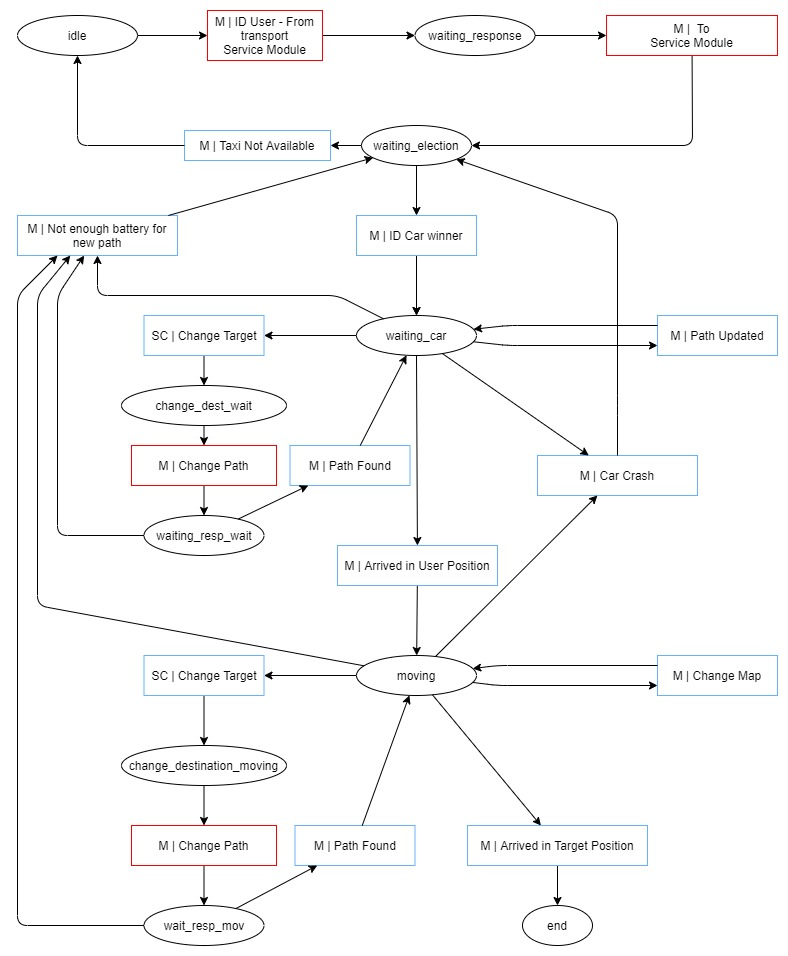
\includegraphics[width=15cm]{automa_utente.jpg}
	\caption{Rappresentazione degli stati possibili dell'entità utente.}
	\label{fig:automa_utente}
\end{figure}

L'immagine \ref{fig:automa_macchina} rappresenta l'automa degli stati dell'entità macchina.


\begin{figure}[htbp]
	\centering
	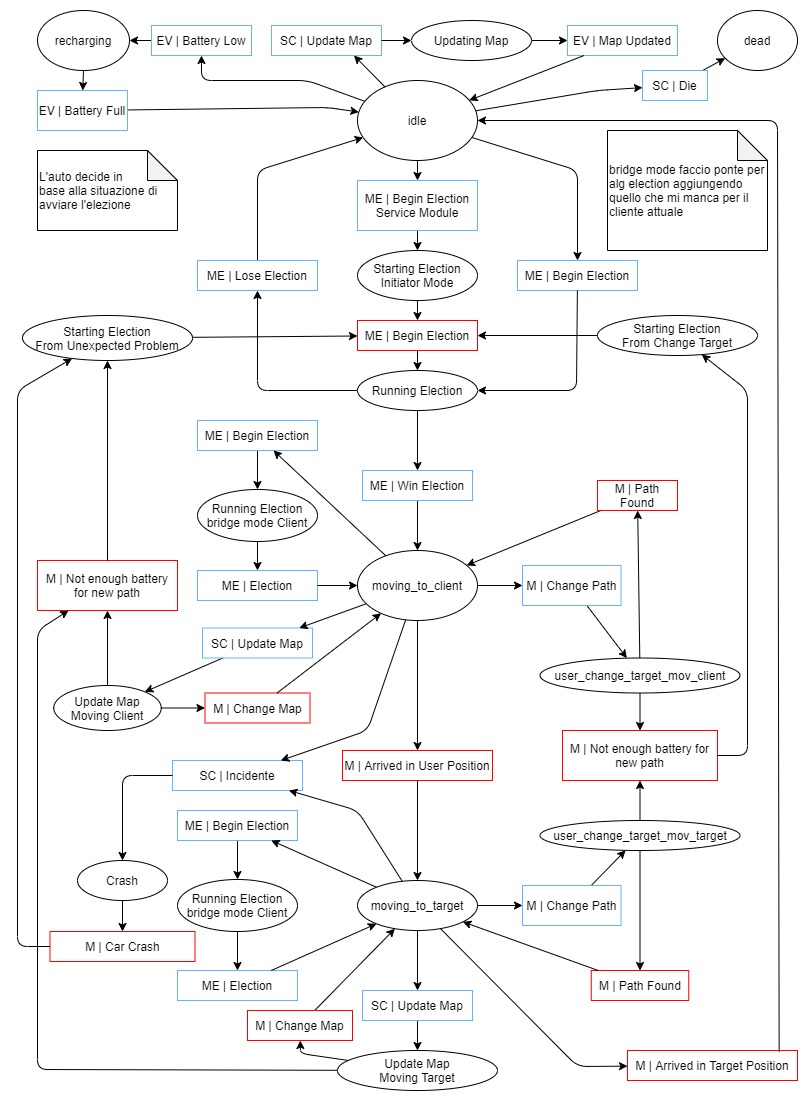
\includegraphics[width=15cm]{automa_macchina.jpg}
	\caption{Rappresentazione degli stati possibili dell'entità macchina.}
	\label{fig:automa_macchina}
\end{figure}

\newpage

\section{Protocolli e algoritmi}
In questa sezione vengono discusse le comunicazioni tra le diverse componenti e gli algoritmi utilizzati all'interno del sistema.

\subsection{Funzioni di costo delle macchine} \label{funzioni_di_costo_macchine}
Per la scelta della macchina più adatta, vengono considerati i seguenti parametri.

\begin{itemize}
	\item Crdt = Carica Rimanente Dopo Trasporto dell'utente.
	\item Cc = Costo Cliente, esprime dopo quanto tempo la macchina raggiungerebbe il cliente.
	\item Cr = Carica Rimanente espressa in unità di misura della distanza percorribile.
	\item Prc = Percorso Rimanente Cliente espresso in unità di misura della distanza assumendo che il taxi sia occupato.
	\item Pvcn = Percorso Verso Cliente Nuovo a partire dalla posizione dopo lo scorso cliente espresso in unità di misura della distanza.
	\item Pvdc = Percorso Verso Destinazione Cliente a partire dalla posizione attuale del cliente espresso in unità di misura della distanza.
	\item Pvcr = Percorso Verso Colonnina Ricarica per permettere alla macchina di ricaricarsi dopo il trasporto se necessario.
\end{itemize}

\begin{equation} \label{funzione_costo_raggiungimento_cliente}
Cc = Prc + Pvcn
\end{equation}

\begin{equation} \label{carica_rimanente_trasporto}
Crdt = Cr - (Cc + Pvdc + Pvcr)
\end{equation}

La scelta della macchina, verrà effettuata minimizzando il tempo del cliente \ref{funzione_costo_raggiungimento_cliente} e, in caso di parità, massimizzando la carica rimanente dopo il trasporto \ref{carica_rimanente_trasporto}. Nel caso in cui non sia univoco il vincitore, la selezione diventa casuale tra i contendenti.

\subsection{Pacchetti scambiati per l'elezione}\label{descrizione_pacchetto}
Vengono utilizzati tre tipi di pacchetti per l'algoritmo di elezione:
\begin{itemize}
	\item Inizio algoritmo elezione
	\item Risultati dei calcoli
	\item Notifica Vincitore
\end{itemize}

\subsubsection{Inizio algoritmo}
Lo scopo di questo pacchetto è di notificare ai nodi raggiungibili dal nodo corrente l'inizio dell'elezione. Esso è formato in questo modo:

\begin{lstlisting}
[ID_self, begin_election, TTL]
\end{lstlisting}

\begin{itemize}
	\item ID\_self: il riferimento a sé stesso per permettere l'impostazione del genitore agli altri nodi raggiunti.
	\item TTL: Per evitare di dover visitare tutto il grafo delle comunicazioni tra le macchine, si è scelto di impostare un TTL al pacchetto affiché dopo un certo numero fisso di salti ci si fermi. Questo porta al fatto che non è garantito che la soluzione trovata sia quella ottimale, tuttavia ciò permette un compromesso tra una buona soluzione e una limitazione della possibile congestione dei messaggi. Inoltre permette una riduzione dei possbili conflitti tra diverse leader election.
\end{itemize}

Il sistema si aspetta che alla ricezione di questo messaggio, il nodo risponda con una notifica di acknowledgment, in tal modo il nodo inviante è sicuro che esso sia stato ricevuto.

\subsubsection{Risultato dei calcoli} \label{pacchetto_calcolato}
Questo pacchetto contiene i dati calcolati dai nodi raggiunti dal pacchetto "inizio algoritmo" assieme a quelli del nodo corrente. Esso verrà poi inviato al genitore e sempre tramite esso è possibile creare la tabella di routing dei nodi coinvolti nell'elezione. Tuttavia per la comunicazione del vincitore, non verrà utilizzata la suddetta tabella poiché è più efficiente effettuare un multicast.

\begin{lstlisting} 
[{ID_1, Cc_1, Crdt_1}, ..., {ID_N, Cc_N, Crdt_N}]
\end{lstlisting}

Esso contiene, in ordine, per ogni nodo i: 
\begin{itemize}
	\item ID\_i: riferimento al veicolo i.
	\item Cc\_i, Crdt\_i: i costi della macchina i come descritto nella funzione di costo \ref{funzioni_di_costo_macchine}
\end{itemize}

\subsubsection{Notifica Vincitore}\label{pacchetto_vincitore}
Scopo del pacchetto è di notificare il vincitore dell'elezione e rilasciare i nodi coinvolti in essa. Questo pacchetto è formato nel seguente modo:

\begin{lstlisting}
[ID_WINNER, winner]
\end{lstlisting}

Il nodo iniziatore lo crea e lo invia in multicast a tutti i nodi coinvolti nell'elezione.

\subsection{Creazione dello Spanning Tree}

Per l'elezione è necessaria la creazione di uno Spanning Tree dei nodi partecipanti ad essa per le comunicazioni. L'Echo algoritm che viene utilizzato ne permette la creazione man mano che i nodi ricevono i messaggi di inizio elezione.

Ogni nodo che partecipa riceve dal genitore padre la notifica di inizio elezione e in tal modo viene creata una relazione padre-figlio tramite la quale possono comunicare. Se un nodo riceve lo stesso tipo di notifica ma possiede già un padre, risponde al mittente di non poter partecipare e non inoltra ai propri vicini la notifica.

La radice dello spanning tree è il nodo iniziatore.

\subsection{Algoritmo di Elezione}
Come già accennato nell'introduzione al punto \ref{intro_algo}, l'algoritmo di elezione scelto è di tipo Wave e ne soddisfa le notorie proprietà. In particolare, si è optato per un Echo algoritm poichè il grafo su cui deve essere applicato è indiretto ed è possibile che siano presenti dei cicli.
L'algoritmo segue i seguenti passi:
\begin{enumerate}
	\item La macchina iniziatrice, la quale viene scelta perché la più vicina al cliente oppure in seguito a degli eventi di aggiornamento della mappa o incidente, inizia la wave creando un pacchetto da inviare ai propri vicini formato come già descritto al punto \ref{descrizione_pacchetto}, poi calcola i propri costi come descritto nella parte \ref{funzioni_di_costo_macchine}, ed aspetta i dati dei nodi che hanno risposto in modo positivo con l'acknowledgment al pacchetto di inizio elezione.
	\item Ogni nodo che riceve il pacchetto di inizio elezione, se non sta già partecipando a un'altra elezione, si sposta nello stato relativo al calcolo del leader. In ogni caso, risponde al nodo inviante se partecipa oppure no all'elezione. In caso negativo, non inoltra il pacchetto di inizio elezione ricevuto ai suoi vicini. In caso positivo, invece, se il TTL è superiore a 0, ne riduce il valore di un'unità e lo inoltra ai propri vicini. Successivamente, come per il nodo padre, si mette in attesa degli ack dei vicini.
	\item Il nodo che riceve il pacchetto di starting election con TTL pari a zero, dopo avere inviato l'ack al genitore, non inoltra ulteriormente l'inizio dell'elezione ai vicini.
	\item Ogni nodo, dopo aver ricevuto l'ack da parte dei figli alla partecipazione dell'elezione, calcola i propri costi e si mette in attesa che i propri figli, se presenti, gli mandino i costi calcolati. Alla ricezione di tutti i costi dei figli esso crea un pacchetto unico concatenando i costi ricevuti al proprio. Successivamente inoltre il pacchetto risultate al padre. Per la struttura di esso si faccia riferimenti a \ref{pacchetto_calcolato}.
	\item Dopo aver inviato al padre i dati relativi ai costi, ogni nodo si mette in attesa di conoscere chi è il leader.
	\item Quando il nodo iniziatore riceve tutti i dati calcola il leader in base alle proprietà descritte nella parte \ref{funzioni_di_costo_macchine}. 
	\item Infine l'iniziatore invia il messaggio contentente il leader in multicasting a tutti i partecipanti all'elezione. Si faccia rifermento alla parte \ref{pacchetto_vincitore} per la descrizione del pacchetto.
	\item Tutti i nodi ricevono la notifica del leader e in base al risultato compiono le azioni più opportune. In ogni caso escono dallo stato di elezione eliminando tutte le informazioni calcolate.
\end{enumerate}

Un esempio dei pacchetti scambiati durate l'algoritmo è presente all'immagine \ref{fig:messaggi_macchina_elezione}. La parte in basso a sinistra mostra lo spanning tree creato.

\begin{figure}[htbp]
	\centering
	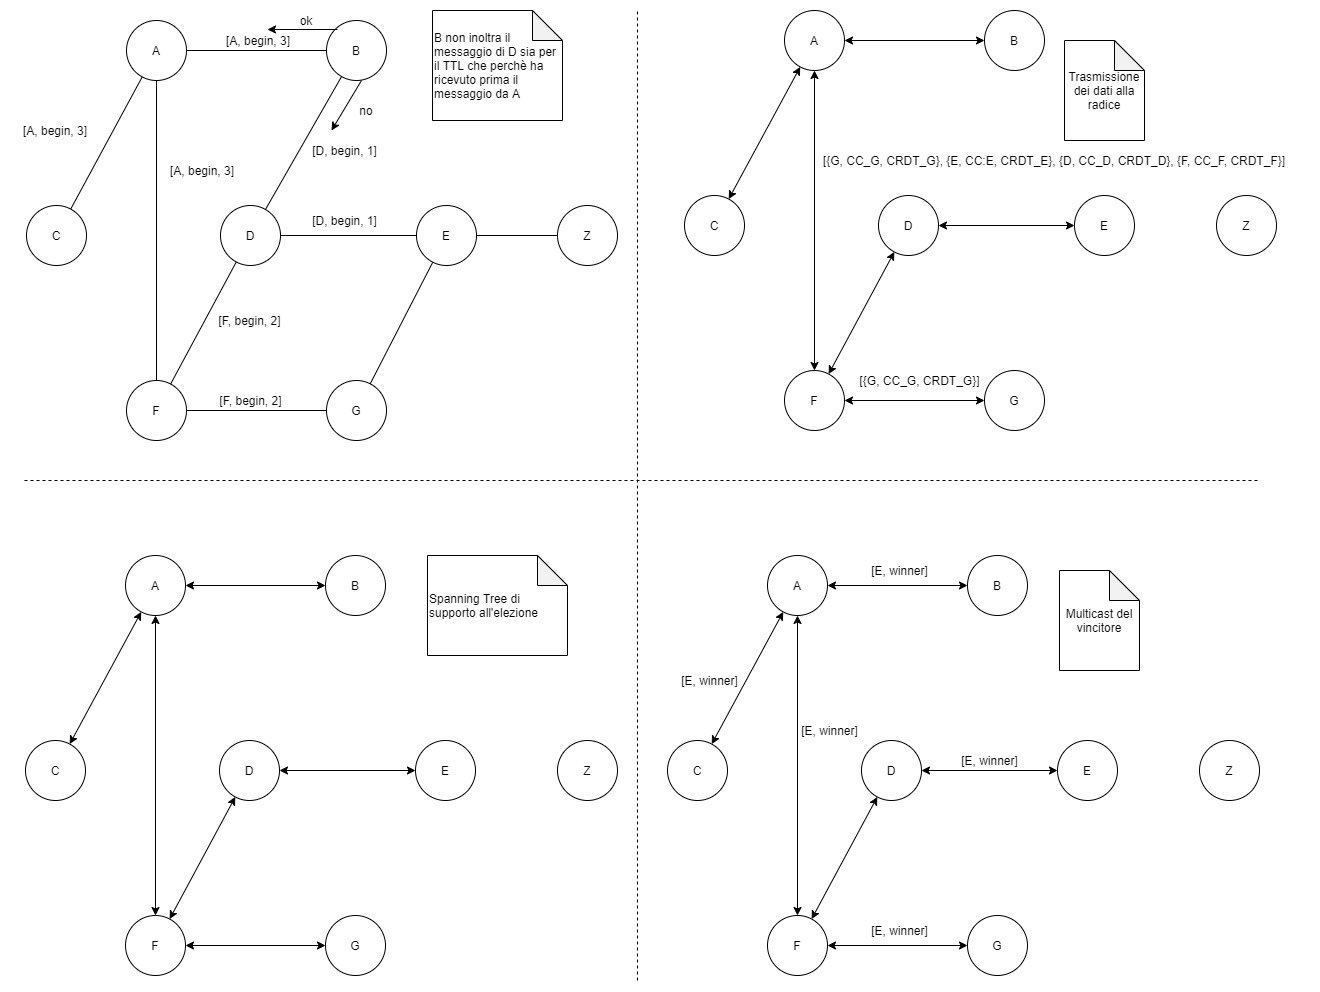
\includegraphics[width=15cm]{messaggi_macchina_elezione.jpg}
	\caption{Rappresentazione dei messaggi scambiati durante l'elezione.}
	\label{fig:messaggi_macchina_elezione}
\end{figure}

\newpage

\subsection{Possibili errori durante l'elezione}

I problemi durante l'esecuzione dell'algoritmo nel sistema sono i seguenti:
\begin{itemize}
	\item Aggiornamento della mappa.
\end{itemize}

I problemi possibili ma assenti per via dell'implementazione del sistema sono i seguenti:
\begin{itemize}
	\item Rimozione di una macchina
	\item Perdita di pacchetti
\end{itemize}

\subsubsection{Aggiornamento della mappa}
Viene discussa nella sezione Aggiornamento Mappa \ref{aggiornamento_mappa}.

\subsubsection{Rimozione di una macchina}
Sebbene il sistema venga costruito in modo che un nodo possa essere rimosso solamente se si trova nello stato "idle", è bene gestire i casi in cui l'eliminazione avvenga in ogni possibile stato, compresa l'elezione. Per risolvere il problema di attesa della risposta da un nodo ormai rimosso, ogni nodo invia dei messaggi di tipo "hello" per controllare lo stato del nodo collegato. In tal modo se non ricevono risposta entro un tempo ragionevole lo considerano rimosso e continuano l'algoritmo di elezione.

\subsubsection{Perdita di pacchetti}
Nel caso in cui vengano persi dei pacchetti durante qualsiasi fase dell'elezione, è possibile accorgersene poichè non ritornano i messaggi di ack. Una possibile soluzione per questo problema è l'utilizzo del protocollo TCP.

\subsection{Aggiornamento della mappa}\label{aggiornamento_mappa}

Questa casistica comporta che i percorsi calcolati, nel caso utilizzino degli archi deprecati, non siano più validi. 

L'aggiornamento può avvenire in diversi momenti e stati della macchina. 

\begin{itemize}
	\item Macchina in stato IDLE: Semplice aggiornamento, non comporta alcun problema.
	\item Macchina in stato Running Election: al termine dell'elezione effettua l'aggiornamento. Se risulta vincitrice ed è necessario, ricalcola il percorso.
	\item Macchina in stato Moving to Client o Moving to Target con un solo cliente: il veicolo effettua l'aggiornamento della mappa e, se necessario, ricarcola il percorso. Se è in grado di soddisfare l'utente, lo notifica del ritardo e torna nello stato precedente. Altrimenti notifica l'utente e inizia una leader election per l'utente.
	\item Macchina in stato Moving to Client o Moving to Target con più clienti in coda: Effettua l'aggiornamento e calcola il massimo percorso che riesce a soddifare con la carica rimanente. In tal modo, nel caso in cui alcuni clienti non possano venir soddifatti li notifica con un messaggio di avviare autonomamente una nuova richiesta al sistema e li rimuove dalla coda. In questo caso non parte alcuna leader election. Nel caso peggiore in cui non riesca a soddisfare nemmeno il cliente corrente l'approccio è come al punto precedente.
	\item Macchina in stato Running Election Bridge Mode: come detto precedentemente, esegue comunque il calcolo del leader e poi si comporta in base al numero di utenti in coda.
\end{itemize}

\subsection{Diagrammi di sequenza dei messaggi}
All'appendice \ref{messaggi_scambiati_appendix}, sono presenti i diagrammi di sequenza dei messaggi che vengono scambiati tra i diversi moduli per permettere le funzionalità del sistema.

\begin{itemize}
	\item Movimento del taxi alla posizione dell'utente e successivo trasporto \ref{fig:messaggi_utente_trasporto}.
	\item Richiesta da parte dell'utente del servizio di trasporto \ref{fig:messaggi_utente_chiede_macchina}.
	\item Richiesta di cambiamento di destinazione da parte dell'utente mentre il taxi è in viaggio verso l'utente \ref{fig:messaggi_utente_cambio_direzione_waiting}.
	\item Richiesta di cambiamento di destinazione da parte dell'utente mentre il taxi lo sta trasportando \ref{fig:messaggi_utente_cambio_direzione_moving}.
	\item Partecipazione all'elezione di una macchina non iniziatrice \ref{fig:messaggi_macchina_partecipazione_elezione}. Poiché è possibile che la macchina si trovi in diversi stati mentre viene avviato l'algoritmo di elezione, sono stati rappresentati tre possibili scenari.
	\item Incidente di una macchina con conseguente notifica all'utente e ricerca di un taxi alternativo \ref{fig:messaggi_macchina_crash}.
	\item Ricarica della macchina, rimozione della macchina dal sistema e aggiornamento della mappa  \ref{fig:messaggi_macchina_batteria_morte_mappaIdle}. In queste operazioni si considera che la macchina sia nello stato 'idle'.
	\item Aggiornamento della mappa della città mentre il taxi si sta muovendo verso il cliente \ref{fig:messaggi_macchina_aggiornamento_mappa_to_client}.
	\item Aggiornamento della mappa della città mentre il taxi sta trasportando il cliente a destinazione \ref{fig:messaggi_macchina_aggiornamento_mappa_to_target}.
	\item Aggiornamento della mappa della città mentre il taxi è occupato con un utente e ne ha altri nella coda \ref{fig:messaggi_macchina_aggiornamento_mappa_clienti}.
\end{itemize}


\section{Architettura fisica e Distribuzione}
Per l'implementazione fisica del progetto, è necessario che ogni automobile elettrica sia dotata di una scheda Wi-Fi per la comunicazione con i veicoli vicini. Il cliente per poter comunicare con il sistema necessita di utilizzare un'applicazione dedicata per le prenotazioni. Si suppone esista già la mappa della città nel formato adatto, ogni automobile deve possederne una copia nel disco locale. Un altro requisito hardware è che le macchine dispongano di sufficiente potenza di calcolo per effettuare velocemente il calcolo dei percorsi.

% Which nodes and platforms involved, and where each component is deployed.

\section{Piano di Sviluppo}
% Since it is diffcult to predict just how hard implementing a new system will be, you should formulate as a set of "tiers", where the basic tier is something youre sure you can complete, and the additional tiers add more features, at both the application and the system level.

Sono stati individuati due insiemi di funzionalità che è necessario supportare.
\subsection{Funzionalità Base}

\begin{enumerate}
%	\item Panino alla guida
	\item Comunicazione peer to peer per la leader election.
	\item Richiesta dell'utente di trasporto.
	\item Gestione della ricarica delle macchine.
	\item Cambio di direzione di utente singolo.
	\item Gestione degli incidenti sia delle macchine che delle strade rotte.
\end{enumerate}

\subsection{Funzionalità Aggiuntive}

\begin{itemize}
	\item Perdita delle connessioni mentre si elegge il leader.
	\item Partecipazione della macchina già impegnata alla leader election.
	\item Possibilità di rimuovere la prenotazione
	\item Possibilità di cambiare destinazione anche se ci sono altri utenti nella coda della macchina candidata
	\item Lista di possibili taxi in caso di pareggio tra i candidati.
	\item Car sharing fino a tre persone.
\end{itemize}

\subsection{Ordine di sviluppo}
Lo sviluppo dell'applicazione verrà suddiviso in diverse versioni via via estese con le nuove funzionalità. In particolare si seguirà questo ordine:

\begin{enumerate}
	\item Ogni macchina potrà parlare con tutte le altre macchine; l'utente invia la richiesta di trasporto alla macchina più vicina a lui; se un veicolo è impegnato con un cliente non partecipa alla selezione del leader per il trasporto; la comunicazione tra i veicoli è diretta, quindi ogni taxi può parlare con chiunque.
	\item Vengono aggiunte le colonnine di ricarica, alle quali le macchine devono far rifornimento se hanno esaurito le batterie; le macchine possono guastarsi; l'utente può decidere di cambiare destinazione.
	\item Rottura delle strade ma senza disconnessione del grafo stradale.
	\item Le connessioni tra le macchine possono perdere andare perse mentre si elegge il leader.
	\item Le macchine possono comunicare solo con quelle vicine.
	\item La macchina partecipa all'elezione anche se al momento è già impegnata, tuttavia si considera disponibile solo dopo aver compiuto il tragitto già attivo.
	\item Implementazione del car-sharing fino a 3 clienti.
	\item Rimuovere prenotazione.
	\item Cambio direzione anche se in lista.
	\item Viene fornita al cliente una lista di possibili candidati vincitori.
%	\item panino alla guida
\end{enumerate}
%!TEX TS-program = pdflatex
%!TEX root = progetto_finale.tex
%!TEX encoding = UTF-8 Unicode

\chapter{Implementazione}

\section{Automi} \label{implementazioneAutomi}
Per l'implementazione degli automi è stata utilizzato ``gen\_statem'', il behavior erlang che semplifica la costruzione di macchine a stati finiti guidate da eventi. Questo behavior è un framework con numerose primitive riguardanti questi costrutti: invio e ricezione di eventi sincroni o asincroni, impostazione di timer e molto altro. Gli automi discussi in \ref{automi} sono stati implementati in modo relativamente veloce potendosi concentrare quasi esclusivamente sulla logica del loro funzionamento piuttosto che sui dettagli implementativi, nascosti appunto dal suddetto framework. 
Qui di seguito si riporta un link alla documentazione ufficiale del framework: \url{https://erlang.org/doc/man/gen_statem.html}.

I sorgenti sono stati opportunatamente commentati per descrivere il funzionamento del codice ma è opportuno compiere una descrizione generale di questi automi, soffermandosi sulle scelte implementative effettuate.

Gli automi implementati rispettano fedelmente gli schemi mostrati \ref{automi}, fatta eccezione per alcune mancanze e piccole modifiche che verranno ora elencate

\begin{itemize}
	\item Negli schemi progettuali si mostrava come la comunicazione fra automi interni a un'automobile non avvenisse mai in modo diretto, infatti l'ascoltatore del mezzo si comportava da proxy fra i due automi. Questa scelta progettuale è stata rivista in fase di implementazione, infatti si è ritenuto più veloce permettere una comunicazione diretta, ottenendo anche un codice più snello, pulito e dal comportamento più chiaro. 
	La comunicazione fra un automa interno al veicolo e un automa esterno, come per esempio fra l'automa dell'elezione e l'applicazione utente, avviene tuttavia usando l'ascoltatore come proxy, il quale infatti è l'interfaccia col mondo esterno per un veicolo. Questo ha permesso di diminuire le dipendeze fra i diversi automi: un automa esterno al mezzo deve conoscere soltanto l'ascoltatore per poter comunicare con il veicolo e tutte le sue istanze.
	\item Negli schemi progettuali erano stati inseriti molti stati che non presentano una controparte nel codice, questi erano stati definiti in fase di progettazione per chiarire le idee sui comportamenti degli automi, o per rendere gli schemi più espressivi, ma non si è ritenuto utile o conveniente inserirli nella loro implementazione. Il comportamento degli automi non è stato tuttavia intaccato dall'eliminazione di questi stati. 
	\item Similmente agli stati, alcuni eventi riportati negli schemi progettuali non presentano una controparte "esatta" negli automi, nel senso che i nomi di questi eventi sono stati ridefiniti in fase implementativa trovando alternative più espressive o, in generale, migliori per le esigenze del codice. Anche in questo caso il comportamento non è stato intaccato ed è possibile trovare un isomorfismo fra i nomi degli eventi inseriti negli schemi e quelli inseriti nel codice.
	\item Per la temporizzazione, in fase di progettazione, si faceva riferimento all'uso di orologi interni, i quali scandivano il tempo attraverso l'uso dei più volte citati ``Tick''. Questo è stato implementato con il modulo gestione tempo sopra mostrato \ref{modules} tuttavia per alcuni particolari casi si è preferito utilizzare i timer del behavior ``gen\_statem''. La preferenza nell'uso dei due strumenti dipende dal particolare caso ma gran parte del codice usa i Tick per la temporizzazione.
\end{itemize}

\subsection{Struttura generale} \label{strutturaGeneraleAutomi}
I diversi automi implementati presentano tutti uno stato interno, inteso come una propria memoria che varia durante l'esecuzione, ed è importante non confondersi con lo stato della macchina a stati finiti, la similitudine fra i due termini si presta a diversi fraintendimenti e d'ora in poi si userà il termine ``memoria'' per indicare lo stato con questa accezione. La memoria di ogni automa è stata modellata definendo un record specifico, il quale aggrega tutti i dati necessari.

Il codice dei diversi automi è organizzato con una struttura molto simile che si può schematizzare in queste 5 sezioni:

\begin{enumerate}
	\item Codice per l'importazione di metodi da moduli esterni,importazioni di costanti definite esternamente, esportazione di metodi, definizione di costanti utilizzate solo localmente.
	\item definizione del record specifico per l'automa: secondo quanto detto ne modella la sua memoria.
	\item elenco dell'API dell'automa: inteso come le funzionalità della sua interfaccia, esportate per essere usate da altri automi.
	\item funzioni dell'automa: ricalcano gli stati dell'automa e i possibili comportamenti a seguito della ricezione dei vari eventi, ogni funzione inserita in questa sezione rappresenta una combinazione stato automa-evento ricevibile in quello stato, la logica dell'automa è raccolta in questa sezione.
	\item funzioni interne: usate localmente.
\end{enumerate}

Ogni automa nel codice ha questa suddivisione e i file col codice sono stati opportunatamente marcati con dei commenti per enfatizzare questa struttura. Ulteriori commenti sono stati sparpagliati nel codice per semplificarne la comprensione, in particolar modo sono stati definiti dei contratti nei metodi delle API.

\subsection{Eventi Globali - la funzione ``handle\_common''} \label{eventiGlobaliAutomi}
In questa sezione si descrive come sono stati gestiti gli eventi globali negli automi, ossia eventi che possono essere ricevuti in stati diversi dell'automa. Come descritto sopra, la sezione 4 del codice raccoglie le funzioni che descrivono la logica dell'automa, il behavior ``gen\_statem'' e il pattern matching di Erlang garantiscono che, se l'automa si trova in un certo stato e riceve un particolare evento, verrà eseguita la funzione insrita in questa sezione che rappresenta la particolare combinazione stato-evento; questa, eventulamente, modificherà la memoria del processo e/o  effettuerà un cambiamento di stato. 
Qui viene riportato un frammento di codice che mostra una di queste funzioni: 

\begin{lstlisting}
waiting_car_queued(cast, taxiServingYou, State) ->
	{next_state, waiting_car, State};
\end{lstlisting}

Si noti come il secondo parametro della funzione indichi il nome dell'evento che triggera l'esecuzione del codice, mentre il nome della funzione indica lo stato.

Gli eventi globali portano a un ovvio overhead se implementati in questo modo, infatti per un evento ricevibile in N stati è necessario scrivere N funzioni diverse, se il comportamento è lo stesso in tutti gli stati questo comporta la scrittura di N funzioni tutte uguali ottenendo ulteriormente numerose dipendeze.

Grazie alle comode primitive Erlang si può definire una sola funziona che gestisca lo stesso evento per stati diversi, nel progetto in esame questa è stata chiamata ``handle\_common''. Nella sezione 4 di quasi tutti gli automi, in testa, sono state definite diverse funzioni ``handle\_common'' che adempiono, appunto, a questo scopo. Ne viene qui riportato un esempio;

\begin{lstlisting}
%ricezione del comando di terminazione
handle_common(cast, {die}, _OldState, State) ->
	PidGpsModule = State#appUserState.pidGPSModule,
	gps_module:end_gps_module(PidGpsModule),
	gen_statem:stop(self());
\end{lstlisting}

Queste funzioni hanno una firma diversa in base all'evento: l'atomo inserito come secondo parametro della funzione indica quale evento ``triggera'' l'esecuzione di quel codice.

\subsection{automa elezione}

Si vuole in questa sezione descrivere un particolare automa del progetto ossia quello relativo all'algoritmo di elezione del taxi candidato...

%!TEX TS-program = pdflatex
%!TEX root = progetto_finale.tex
%!TEX encoding = UTF-8 Unicode

\chapter{Validazione}

Check if requirements from Chapter 2 have been fullfilled. Quantitative tests (simulations) and screenshots of the interfaces are put here.

\section{Compilazione ed esecuzione del codice}

Istruzioni per la compilazione ed esecuzione
Scompattare il contenuto della cartella in una posizione a scelta. 
Avviare erlang e posizionarsi all'interno della root del progetto. 
Se assente, creare la cartella ``ebin'' sempre nella root.
Eseguire il comando
\lstinline|make:all().|
Spostarsi nella cartella "ebin" tramite il comando
\lstinline|cd("ebin").|
Avviare l'environment tramite il comando
\lstinline| PID_ENV = main:start_project().|
Viene avviato l'environment 


\section{Test eseguiti}

\section{Controllo requisiti}

\chapter{Implementazione}

Il linguaggio scelto per l'implementazione del progetto è Erlang. Esso è stato selezionato per diversi motivi tra cui: fornisce nativamente il supporto alla gestione di messaggi e scambio di essi tra diverse entità; permette di creare in poche righe di codice diversi beam a cui poter richiedere dei servizi; fornisce librerie tramite le quali è possibile creare facilmente gli automi e le interazioni fra essi. Inoltre supporta nativamente la programmazione concorrente semplificando la gestione da parte dello sviluppatore della programmazione parallela. Infine essendo un linguaggio funzionale, che quindi non presenta memoria condivisa, non permette l'esistenza della race condition tra processi.

In questo progetto non utilizzate piattaforme esterne di alcun genere poiché si assume che l'autenticazione tra utente e applicazione per il servizio sia già stata effettuata.

Essendo un'architettura peer to peer, non è necessaria alcuna piattaforma a parte l'autenticazione cliente - servizio.

\section{Generazione dell'ambiente virtuale}
Il problema della modellazione di una città è stato risolto con un grafo pesato connesso non orientato: si assume che se due nodi sono connessi è perché vi è una strada tra di essi ed è bidirezionale. Il peso indica quanto costa attraversarla. 

\subsection{Entità presenti}
Si immagina che i diversi nodi siano posizionati all'interno di un piano cartesiano, pertanto possiedono delle coordinate che ne indicano la posizione. Questo permette di capire la distanza tra di essi e quindi se diverse entità riescono a comunicare tra di loro.

\subsection{Componenti del grafo} \label{componenti_grafo_citta}
Ogni nodo del grafo possiede quattro proprietà:
\begin{itemize}
	\item attributo nome: generato del tipo ``aa'', ``ab'', ``ac'', ... incrementale per ogni nodo.
	\item attributo id: numero incrementale per ogni nodo a partire da 0. Utilizzato per la definizione del grafo della città.
	\item Coordinate X e Y: definiscono la posizione del nodo all'interno del piano cartesiano rappresentante la città.
\end{itemize}

Per quanto riguarda gli archi, essi posseggono tre proprietà:
\begin{itemize}
	\item ID\_Nodo\_1 - ID\_Nodo\_2: indica quali nodi collega.
	\item Peso: indica il peso dell'arco, calcolato in funzione della distanza tra i nodi che collega l'arco.
\end{itemize}

Infine vengono selezionati alcuni nodi tra quelli del grafo che conterranno le colonnine di ricarica. Per far questo è stato applicato il seguente algoritmo:
\begin{enumerate}
	\item In base al numero totale delle colonnine, il piano cartesiano viene suddiviso in parti uguali.
	\item Selezione di un nodo casuale all'interno della parte creata a cui assegnare la colonnina.
\end{enumerate}

\subsection{Parametri per la generazione}
Il linguaggio utilizzato per la generazione della città è python. All'interno del file ``map\_generator'' è possibile impostare i diversi parametri per la generazione della città, vale a dire:
\begin{itemize}
	\item WEIGHT\_MIN: Peso minimo degli archi.
	\item WEIGHT\_MAX:  Peso massimo degli archi.
	\item TOTAL\_NODES: Totale numero di nodi del grafo.
	\item TOTAL\_EDGES:  Totale numero di archi del grafo.
	\item TOTAL\_CHARGING\_COLS:  Totale numero delle colonnine di ricarica nel grafo.
	\item CARTESIAN\_SIDE:  Lato del quadrato cartesiano utilizzato per la mappa.
\end{itemize}

Per quanto riguarda il numero di colonnine, esso non è garantito essere rispettato per il seguente motivo: come spiegato precedentemente, l'algoritmo utilizzato suddivide il piano in parti uguali ma potrebbe capitare nel caso esse siano piccole che non vi sia alcun nodo all'interno. Dato che in ogni zona è presente al più una colonnina, può capitare che non siano presenti zone con nodi liberi a cui assegnare le rimanenti.

\subsection{File generati}
Lo script in python crea cinque file:
\begin{itemize}
	\item ``map.pdf'': I dati generati per il grafo vengono esportati nel formato dot e da esso viene generato questo file al cui interno è presente una rappresentazione visuale del grafo: sono presenti i nodi con le proprietà descritte precedentemente e gli archi con delle etichette rappresentanti il loro peso. Un esempio del pdf prodotto è l'immagine \ref{fig:esempio_citta_dot}.
	\item ``map.png'': Rappresentazione visuale delle posizioni dei nodi all'interno del piano cartesiano. I nodi colorati di rosso sono quelli contenenti le colonnine di ricarica. Un esempio del png prodotto è l'immagine \ref{fig:esempio_citta_png}.
	\item ``city\_map\_nodes.dat'': file testuale contenente i dati dei nodi formattati in modo da essere compatibili con la struttura creata in erlang. Un esempio è il seguente:
	\begin{lstlisting}
		10
		a 0 1 4
		b 1 2 12
		c 2 3 12
		d 3 3 16
		e 4 5 2
		...
	\end{lstlisting}
	\item ``city\_map\_graph.dat'': file testuale contenente i dati del grafo formattato in modo da essere compatibile con la libreria utilizzata in erlang. Un esempio è il seguente:
	\begin{lstlisting}
		10 30 undirected d
		6 0 17
		0 1 12
		1 8 18
		8 4 20
		4 7 14
		7 3 21
		3 9 18
		...
	\end{lstlisting}
	\item ``city\_map\_charging\_cols.dat'': file testuale contenente i dati dei nodi delle colonnine. Essi sono formattati in modo da essere compatibili con la struttura creata in erlang. Lo stile è il medesimo del file ``city\_map\_nodes.dat''.
	
\end{itemize}


\begin{figure}[htbp]
	\centering
	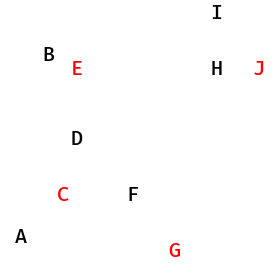
\includegraphics[width=8cm]{esempio_citta_png.jpg}
	\caption{Esempio del posizionamento dei nodi all'interno della città.}
	\label{fig:esempio_citta_png}
\end{figure}

\begin{figure}[htbp]
	\centering
	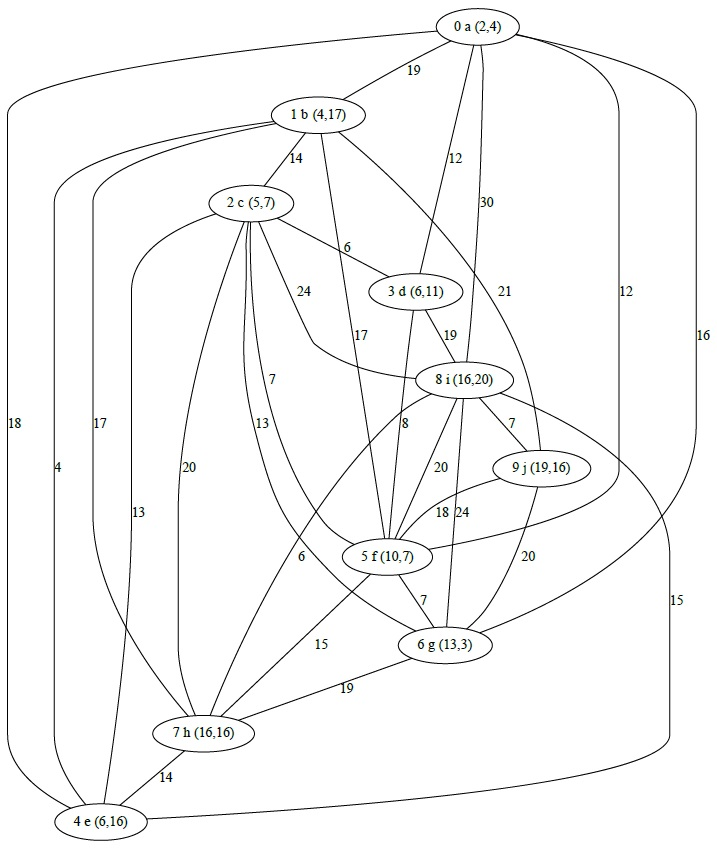
\includegraphics[width=14cm]{esempio_citta_dot.jpg}
	\caption{Esempio di grafo utilizzato per la simulazione della città.}
	\label{fig:esempio_citta_dot}
\end{figure}

\newpage

\section{Entità Ambiente}
Questa entità, chiamata anche ``environment'', rappresenta il mondo in cui avviene la simulazione. Tramite esso è possibile creare entità, rimuoverle e far acccadere eventi.

\subsection{Variabili di stato}
Il suo stato contiene:
\begin{itemize}
	\item cars: lista dei pid delle macchine attualmente presenti nella città. In particolare è memorizzato il pid dell'automa ascoltatore, poichè è ad esso che vengono poi indirizzati i messaggi che riguardano la macchina di cui fa parte.
	\item total\_cars: numero totale delle macchine presenti. Esso viene aggiornato a ogni aggiunta e rimozione.
	\item users: lista dei pid degli utenti presenti nella città. Essa viene aggiornata sia quando l'utente viene creato che rimosso, vale a dire quando è giunto a destinazione.
	\item total\_users: numero totale degli utenti attualmente in città.
	\item cars\_crashed: lista delle macchine attualmente in stato ``crash''.
	\item total\_cars\_crashed: numero totale delle macchine in stato ``crash''.
	\item city: dati della città come descritti nella parte \ref{citta_e_algoritmi}.
	\item pid\_gps\_server: pid del server gps. Ne viene spiegato il funzionamento al punto \ref{gps_server}.
	\item autoEvents: flag che indica se gli eventi automatici sono abilitati oppure no.
	\item tick\_s\_pid: pid dell'istanza tick server dedicata all'environment.
	\item tick\_counter: contatore dei tick ricevuti.
	\item car\_pids: dizionario che associa il nome al pid delle macchine presenti.
	\item last\_car\_id: numero incrementale utilizzato per la generazione del nome delle macchine.
	\item user\_pids: dizionario che associa il nome al pid degli utenti present.
	\item last\_user\_id: numero incrementale utilizzato per la generazione del nome degli utenti.
	\item car\_prefix: prefisso utilizzato per i nomi delle macchine. Nella simulazione è pari a ``c''.
	\item user\_prefix: prefisso utilizzato per i nomi delle macchine. Nella simulazione è pari a ``u''.
\end{itemize}

\subsection{Eventi e gestione di essi}\label{env_events}
Sono stati gestiti sette tipi di eventi. Di seguito l'identificativo dell'evento ed il relativo nome assieme a una minima spiegazione:
\begin{itemize}
	\item -1 Nothing: nulla, lo stato della città resta inalterato.
	\item 1 Spawn car: questo evento causa la creazione di una macchina in un punto casuale della città. La creazione viene discussa nella parte \ref{creazione_distruzione_entita}.
	\item 2 Spawn user: questo evento causa la creazione di un utente in un punto casuale della città con una destinazione random. Maggiori informazioni sono presenti nella parte \ref{creazione_distruzione_entita}
	\item 3 Change target: quando occorre questo evento un utente casuale oppure quello passato per parametro cambierà la propria destinazione se possibile.
	\item 4 Car crash: una macchina scelta casualmente o determinata dal parametro passato passerà dallo stato normale a crash. Maggiori informazioni nella parte RIFERIMENTO\_CAR\_CRASH. Il suo pid viene aggiunto alla lista ``cars\_crashed''. Nel caso venga selezionata una macchina già in quello stato viene stampato un messaggio di errore.
	\item 5 Car fix: una tra le macchine presenti nella ``lista cars\_crashed'' viene selezionata e ripatata tramite l'apposito evento. 
	\item 6 Remove Car: una macchina in stato ``idle'' viene rimossa dalla mappa. Se la macchina selezionata non è in idle si cerca una seconda macchia e via via fino al valore limite della variabile globale ``max\_kill\_tries''. Questo limite è dovuto alla volontà di evitare situazioni di stallo.
\end{itemize}

Nel caso in cui il flag ``autoEvents'' dello stato sia impostato a ``true'', il contatore dei tick ricevuti inizierà ad accumulare il tempo trascorso. In base alla variabile globale ``ticks\_event'' vengono determinati ogni quanti tick ricevuti debba acccadere un evento casuale tra quelli appena discussi.

Tramite le API fornite dal modulo è possibile innescare un determinato evento tramite la funzione ``triggerEvent'' e l'identificativo dell'evento desiderato. In alternativa è possibile utilizzare le funzioni già pronte per gli eventi a cui si può passare i parametri desiderati. Maggiori informazioni sono presenti nella documentazione dei singoli metodi.

\subsection{Creazione ed eliminazione delle entità} \label{creazione_distruzione_entita}
La creazione l'eliminazione di una determinata entità comportano diverse modifiche allo stato dell'environment, pertanto verranno analizzate in modo separato.

Dopo aver creato un'entità è necessario aggiornare il relativo contatore per evitare che esistano entità diverse ma con lo stesso nome.

\subsubsection{Creazione di una macchina}
I dati di cui necessita una macchina sono: posizione di partenza, pid del server gps a cui poter comnicare la propria posizione, mappa della città per poter eseguire l'algoritmo di elezione ed infine nome a lei assegnato. Dopo aver preparato i dati viene eseguita una chiamata al modulo della macchina e il pid ottenuto viene aggiunto alla lista delle macchina attualmente in città. Vengono incrementati i contatori delle macchine in città e dei nomi di esse. Infine viene aggiornato il dizionario che tiene traccia dell'associazione nome-pid macchina.

Il modulo della macchina crea le proprie istanze come spiegato al punto REF\_SPAWN\_MACCHINA

\subsubsection{Creazione di un utente}
I dati di cui necessita un utente sono: posizione di partenza, richiesta di trasporto formata dalle due posizioni di partenza e arrivo, pid del server gps per la propria applicazione e nome dell'utente. Il pid del server gps serve poichè è l'automa utente a creare l'automa ``app\_utente''. Il punto di partenza della richiesta deve essere lo stesso della posizione iniziale dell'utente. In caso contrario viene generato un messaggio di errore. Come per la macchina, anche dopo la creazione dell'utente vengono aggiornate le relative liste.

\subsubsection{Eliminazione di una macchina}
Come già accennato nella parte \ref{env_events}, l'eliminazione di una macchina dall'ambiente avviene solo se essa si trova nello stato di idle. Questa scelta è stata fatta perché simile alla realtà. Una volta individuata, le si invia il segnale di morte e la si rimuove dalla lista delle macchine nell'ambiente. Inoltre viene rimossa la sua coppia nome-pid nel dizionario.

\subsubsection{Rimozione di un utente dall'ambiente}
Quando un utente è giunto a destinazione, esso considera compiuto il proprio dovere ed invoca il metodo dell'environment ``removeUser'' che ne elimina i riferimenti dallo stato come già spiegato per la macchina.

\section{Mappa città e relativi algoritmi} \label{citta_e_algoritmi}
Il record ``city'' contiene cinque parametri:
\begin{itemize}
	\item city\_graph: grafo caricato dalla libreria descritta al punto \ref{libreria_algoritmi}.
	\item total\_nodes: numero totale dei nodi del grafo.
	\item total\_edges: numero totale di archi del grafo.
	\item nodes: nodi presenti nella mappa secondo la struttura definita al punto \ref{nodi_citta}.
	\item column\_positions: sottoinsieme dei nodi che contengono le colonine.
\end{itemize}

Esso contiene lo stato attuale della città dal punto di vista topologico. Le sue componenti vengono utilizzate da diverse entità del sistema per diversi scopi:
L'automa elezione inserire riferimento ne utilizza il city\_graph per calcolare i costi della macchina.

L'entità ambiente inserire riferimento ne utlizza i nodi per generare casualmente le posizion iniziali di macchine e utenti.

Il Gps Server \ref{gps_server} ne utilizza i nodi per creare la propria struttura dove tiene traccia della posizione attuale delle entità presenti in un determinato istante nella città

\subsection{Nodi città}\label{nodi_citta}
Come già descritto al punto \ref{componenti_grafo_citta}, ogni nodo possiede diverse proprietà che vengono memorizzate nell'apposito record definito in questo modo:
\begin{itemize}
	\item name: nome del nodo
	\item id: identificativo numerico del nodo, utlizzato per la sua codifica nel grafo. Questo è necessario poichè la libreria descritta al punto \ref{libreria_algoritmi} per identificare i nodi utilizza il loro id numerico.
	\item pos\_x: coordinata sull'asse delle ascisse del nodo.
	\item pos\_y: coordinata sull'asse delle ordinate del nodo.
\end{itemize}

All'avvio l'entità ambiente, tramite il modulo ``node\_utils'', carica la lista dei nodi presenti nel file ``city\_map\_nodes.dat'' e la lista presente nel file ``city\_map\_charging\_cols.dat''. Queste due liste vengono utilizzate per identificare quali sono i nodi della città e quali di essi sono colonnine. 

La scelta di separarle è stata effettuata poichè nella ricerca della colonnina più vicina alla posizione della macchina è sufficiente calcolare la distanza tra ogni colonnina e il punto desiderato, senza scorrere tutti i nodi della mappa.

Il metodo ``get\_nearest\_col/3'' presente nel modulo ``city\_map'' permette di sapere quale colonnina sia quella più geograficamente vicina al nodo passato come parametro.

Il modulo ``node\_utils'' fornisce i diversi getter per ottenere le informazioni desiderate a partire dalla lista e un identificativo per un determinato nodo. Esso inoltre fornisce dei metodi per ottenere un nodo random presente, con la possibilità di escludere un nodo. Questa proprietà viene utilizzata nella generazione delle richieste degli utentei come spiegato al punto REF\_CREATING\_REQUEST.

\subsection{Libreria per algoritmi} \label{libreria_algoritmi}
Data la natura del progetto, è necessario poter gestire grafi ed applicare ad essi l'algoritmo di Dijkstra per il calcolo dei cammini minimi tra due nodi di esso. Per eseguire questo compito, si è scelto di utilizzare la libreria ``erlang-algorithms'' fornita da Aggelos Giantsios, reperibile al sito \url{https://github.com/aggelgian/erlang-algorithms}. Essa fornisce sia le strutture base che gli algoritmi da applicare ad esse.

Di questa libreria vengono principalmente tre funzionalità:
\begin{itemize}
	\item graph:from\_file/1: permette, leggendo un file, di crearne il grafo associato in un'apposita struttura erlang.
	\item dijkstra:run/2: esegue l'algoritmo di dijkstra applicato al grafo passato come parametro iniziando dal nodo indicato.
	\item graph\_utils:getDataPath/2: vengono passati i risultati calcolati da dijkstra e il nodo target di cui si vuole sapere il percorso calcolato.
\end{itemize}

L'algoritmo di Dijkstra viene utilizzato nell'automa dell'elezione come spiegato al punto REF\_elezione\_automa.

\section{Moduli Gps e Server Gps}
Il problema in esame concerne la posizione delle diverse entità all'interno di una città, pertanto è necessario esse possiedano un modulo in grado di dir loro la posizione e distanza delle altre entità presenti. Per far questo è stato deciso di creare due moduli:
\begin{itemize}
	\item gps\_server: tiene traccia delle posizioni di tutte le entità.
	\item gps\_module: comunica con il server per sapere quali sono le entità vicine a lui.
\end{itemize}

\subsection{Gps Server}\label{gps_server}
Con lo scopo di simulare la ricezione dei vicini delle diverse entità, esso fornisce dei messaggi tramite i quali è possibile ottenere queste informazioni. Questo modulo utlizza quattro record:

\begin{itemize}
	\item nodeDistance: è una tupla formata da due valori, vale a dire ``dist'', che indica la distanza dal nodo che fa la richiesta, e ``entities'', che è una lista di pid. Il significato di essa è ``a questa distanza ci sono queste entità''.
	\item entity: è una tupla formata da tre valori: ``pid'', ossia il pid dell'entità, ``type'', l'atomo che contiene l'informazione sul tipo di entità, ed infine ``position'', che contiene il nome del nodo dov'è attualmente situata l'entità.
	\item nodeEntities: contiene due campi, vale a dire ``nodeData'', che contiene i dati del nodo che si sta considerando (dati come definiti al punto \ref{nodi_citta}), e ``entities'', che è una lista di pid. 
	\item gpsServerState: contiene due liste, una di entity come appena definite e una di nodeEntities.
\end{itemize}

Le funzionalità che offre il server sono principalmente due:

\begin{itemize}
	\item getNearEntities/2: i parametri che riceve sono la posizione di partenza e la potenza del segnale. Ciò che il server fa è il calcolo della distanza di tutti i nodi della mappa dal nodo di partenza e filtra questi in base al valore della potenza del segnale. Non importa l'ordine, l'output è una lista contenente i nodi entro il range che il segnale copre.
	\item getSortedEntities/2: i parametri che riceve sono la posizione di partenza e la potenza del segnale. Il server, dopo aver calcolato la distanza di tutti i nodi e filtrati in base alla distanza massima, li ordina tramite un algoritmo di sorting. L'output è una lista di pid ordinati in base alla distanza dal nodo di partenza ma senza l'informazione della distanza. Sta al richiedente estrarre il pid voluto.
\end{itemize}

In entrambi i casi vengono effettuati i seguenti passaggi: nel calcolo delle distanze, viene creata un'istanza del record ``nodeDistance'' contenente, come già spiegato, distanza e pid presenti nel nodo; poichè i pid delle entità sono presenti in liste diverse, viene applicata la funzione ``packNodes'' che estrae dal record ``nodeDistance'' i pid e ne crea una lista.

\subsection{Gps Module}\label{gps_module}
Rappresenta il modulo ``localizzatore vicini'' descritto nella parte \ref{modules}. Esso fornisce all'automa della macchina e dell'applicazione dell'utente le funzioni per il recupero delle entità vicine.

Il suo stato contiene i seguenti parametri:
\begin{itemize}
	\item pid\_entity: il pd a cui è associato il modulo gps. Nel protetto corrisponde all'applicazione dell'utente oppure all'automa ascoltatore della macchina.
	\item name\_entity: il nome dell'entità di cui fa parte.
	\item pid\_gps\_server: il pid del server gps a cui fare le richieste delle entità vicine.
	\item entity\_type: tipo dell'entità a cui è associato. Nel caso faccia parte di una macchina esso sarà ``car'' mentre nel caso dell'applicazione utente sarà ``user''.
	\item current\_position: nome del nodo attuale dov'è situata l'entità di cui fa parte.
	\item module\_range: potenza del segnale gps del modulo. Viene utilizzato dal gps server per filtrare i risultati come già spiegato al punto \ref{gps_server}.
	\item map\_side: poiché viene assunto che il modulo dell'applicazione utente possa sempre individuare la macchina più vicina, la potenza utilizzata dalla funzione ``getNearestCar'' è pari alla diagonale della mappa, pertanto sicuramente individua tutte le macchine.
\end{itemize}

La funzione ``getNearestCar'' richiede al Gps server le entità presenti ordinate secondo la distanza dal nodo dov'è situato il modulo gps e, dopo aver rimosso il pid relativo a alla propria entità, ne seleziona il primo elemento. 

La funzione ``getNearCars'' esegue come la precedente la richiesta al server indicando la propria posizione e il proprio livello di segnale. La risposta del server, dopo aver rimosso da essa il pid relativo all'entità di cui il modulo fa parte, viene inoltrata all'entità che ha eseguto questa funzione.

\section{Automa Elezione}
Il principale problema affrontato in questo progetto è stato quello di eleggere quale sia la migliore macchina per soddisfare la richiesta dell'utente. Come già accennatto precedentemente al punto REF\_AUTOMI\_IMPLEMENTAZIONE, ogni macchina possiede un'istanza di questo automa.

\subsection{Record utilizzati}\label{record_elezione}
Per l'elezione vengono utilizzati diversi record, che per lo più rispecchiano i pacchetti definiti al punto \ref{descrizione_pacchetto}.

\begin{itemize}
	\item user\_request: formato dalla coppia ``from''  e ``to'' indica il punto di partenza e arrivo dell'utente.
	\item dataElectionBegin: creato dall'automa ascoltatore, indica all'elezione di iniziare i calcoli per l'elezione. Al suo interno contine la richiesta dell'utente ed il pid dell'applicazione dell'utente.
	\item dataElectionPartecipate: creato dall'automa elezione, rispecchia la struttura spiegata precedentemente. Contiene: riferimento alla macchina ``padre'' per la successiva comunicazione dei risultati; user request come definita prima; ttl per determinare se inoltrare ulteriormente l'invito.
	\item electionCostData: vengono creati da ogni macchina e contengono il proprio pid per l'eventuale comunicazione del vincitore assieme al CC e CRDT come definiti al punto \ref{funzioni_di_costo_macchine}.
	\item carPartecipate: formato da tre campi, ha lo scopo di mantenere le informazioni dei nodi invitati a partecipare a una determinata elezione. Contiene il pid della macchina invitata, una lista dei costi ad essa associata ed una variabile ``sent results'' che indica se la determinata macchina ha già inviato oppure no i propri calcoli per l'elezione.
	\item election\_result\_to\_car: risultati per la macchina, contengono il pid del vincitore, il pid dell'app dell'utente per la creazione delle relative tappe per l'automa moving e la richiesta in modo che sia più facile popolare la lista ``users in queue'' dell'automa ascoltatore. Maggiori informazioni al punto REF\_USERS\_IN\_QUEUE.
	\item election\_result\_to\_user: risultati per gli utenti, vengono creati dall'automa ascoltatore risultato vincitore dell'elezione. Contengono il pid e nome del taxi vincitore assieme al tempo di attesa per l'arrivo nella posizione dell'utente.
\end{itemize}

\subsection{Varaibli di istanza dell'automa}\label{stato_elezione_automa}
Ogni istanza dell'automa possiede alcune variabili costanti e altre che variano per ogni elezione. Queste sono le variabili comuni a tutte le elezioni:
\begin{itemize}
	\item pidCar: pid dell'ascoltatore della macchina, utilizzata per inviare i messaggi agli altri automi.
	\item nameCar: nome della macchina, utilizzata per i messaggi di stato.
	\item pidMovingCar: pid dell'automa moving, a cui vengono richiesti i dati dell'elezione come discusso al punto REF\_DATI\_ELEZIONE.
	\item pidGps: pid della propria scheda gps, utilizzata per sapere quali siano le macchine vicine.
	\item cityMap: mappa della città, come descritta al punto \ref{citta_e_algoritmi}.
\end{itemize}

Di seguito le variabili utilizzate localmente per un'unica elezione:
\begin{itemize}
	\item flag\_initiator: indica se è questa la macchina iniziatrice dell'elezione, vale a dire quella che dovrà calcolare chi sia il miglior taxi.
	\item pidAppUser: nel caso del nodo iniziatore, si tiene il riferimento all'utente che ha richiesto il trasporto per la successiva comunicazione.
	\item currentRequest: copia della richiesta dell'utente, utilizzata per la generazione del record ``election\_result\_to\_car''
	\item my\_election\_cost: costi calcolati per la macchina che possiede l'elezione. Nel caso essa risulti candidabile equivalgono a una lista contenente i ``electionCostData'' definiti precedentemente, altrimenti una lista vuota.
	\item queueToManage: è una tupla formata da tre campi, i quali sono la coppia costo totale - percorso relativi ai diversi path che la macchina deve compiere per soddisfare un cliente. Sono i dati ``grezzi'' ottenuti dall'applicazione degli algoritmi sui grafi, da elaborare per l'automa moving.
	\item dataToSendPartecipate: è il record ``dataElectionPartecipate'' utilizzato come invito alla partecipazione per gli altri automi elezione.
	\item parent: pid dell'automa che svolge il ruolo di padre durante l'elezione. 
	\item carsInvited: lista dei pid delle macchine invitate alla partecipazione dell'elezione da parte di un determinato modo
	\item childrenPartecipate: elenco di record ``carPartecipate'' che consente di tener traccia dei nodi che partecipano effettivamente all'elezione.
	\item totalCosts: lista dei costi dei nodi figli di un determinato nodo e di quello del nodo corrente.
	\item car\_moving\_queue\_data: elenco dei record creati a partire dalla ``queueToManage'' per l'automa moving.
\end{itemize}

\subsection{Algoritmo di Elezione}
Riprendendo l'algoritmo definito al punto \ref{algoritmo_elezione}, di seguito ne viene analizzata l'implementazione di ogni passo.

\begin{itemize}
	\item Il nodo inizatore riceve dall'automa ascoltatore il messaggio che contiene le informazioni necessarie per l'elezione. 

	\lstinline|{beginElection, dataElectionBegin}|

	Esso quindi calcola i propri costi come spiegato al punto \ref{implementazione_calcolo_costi} e dopo aver richiesto al proprio modulo gps quali siano le entità vicine, aggiorna il proprio stato. Nel caso in cui la lista delle macchine vicine non sia vuota, le invita e si sposta nello stato ``initiator\_final\_state''. Nel caso invece in cui ci siano delle macchine da invitare, prepara il record ``dataElectionPartecipate'' impostando le variabili e il ttl come descritto nella variabile globale ``max\_hops\_election'', lo invia alle macchine da invitare con l'apposito messaggio e si sposta in ``running\_election''.

	\lstinline|{partecipateElection, Data}|
	\item I nodi che ricevono l'invito di partecipazione possono essere di due tipi: nello stato ``idle'' e in un altro stato dell'elezione. Nel primo caso rispondono al nodo che li ha invitati con il messaggio 

	\lstinline |{invite_result, {Self_Pid, i_can_join}}|
	
	per indicare che partecipano attivamente all'elezione. Calcolano i propri costi secondo il metodo \ref{implementazione_calcolo_costi} e controllano il ttl contenuto nell'invito. Nel caso in cui sia maggiore di zero chiedono al modulo gps i propri vicini e inviano loro il messaggio di invito con ttl diminuito di un'unità. Nel caso sia uguale a zero non estendono l'invito di partecipazione. Successivamente si spostano nello stato ``running\_election'' in attesa delle risposte dei nodi invitati. Nel caso invece il nodo sia in uno stato non di ``idle'' è l'ascoltatore ad inviare al nodo richiedente il messaggio

	\lstinline |{invite_result, {Self_Pid, i_can_not_join}}|

	ad indicare la non partecipazione.

	Nel caso non sia necessario l'invito di altre macchine all'elezione, dallo stato idle ci si sposta nello stato ``waiting\_final\_results'' in attesa della comunicazione del vincitore dal parte del nodo iniziatore.
	\item Nello stato ``running\_election'' ogni automa gestisce le due liste precedentemente definite ``carsInvited'' e ``childrenPartecipate''. 
	
	Ogni volta che un nodo in questo stato riceve un messaggio del tipo 
	
	\lstinline |{invite_result, {Self_Pid, Result}}|
	
	cerca il pid ``Self\_Pid'' dalla lista ``carsInvited'' e se lo trova ed il valore della variabile ``Result'' è pari a ``i\_can\_join'' crea un record del tipo ``carPartecipate'' con il campo ``sent\_results'' a ``not\_sended\_results''. Nel caso in cui esso non venga trovato vuol dire che il nodo ha già mandato i propri risultati e quindi è già stato rimosso dalla lista degli invitati.

	Ogni volta che un nodo in questo stato riceve un messaggio del tipo 

	\lstinline |{costs_results, Data}|

	Controlla se il nodo è ancora presente nella lista degli invitati. In caso affermativo lo rimuove, crea il record ``carPartecipate'' con i dati ricevuti e impostando il flag ``sent\_results'' a ``ok'' aggiungendolo alla lista dei partecipanti attivi definita prima. Nel caso in cui non sia presente nella lista degli invitati, lo cerca nella seconda lista e ne aggiorna le proprietà utilizzando come identificativo il pid del nodo.

	In entrambi i casi alla fine viene chiamata la procedura dedicata al calcolo della fine ``running\_election'' che se, la lista degli invitati è vuota e tutti i partecipanti hanno inviato i propri dati, invia i dati al nodo genitore e sposta l'automa nello stato di attesa / calcolo dei risultati dell'elezione.
	
	Per ridurre i calcoli eseguiti da un unico nodo, si è optato per inoltrare al genitore solamente i dati del nodo migliore del proprio sottoalbero. I dati scambiati contenenti le informazio di un particolare nodo sono presenti nei record di tipo ``electionCostData'' come già definito.

	\item Il nodo iniziatore, a differenza dei nodi partecipanti, appena riceve tutte le risposte dai propri figli si sposta nello stato speciale ``initiator final state'' nel quale, dopo l'applicazione della funzione di selezione del miglior dato, crea i risultati dell'elezione. In base ai calcoli effettuati crea il record del vincitore e inoltra il messaggio a tutti i nodi partecipanti all'elezione.
	
	\item Ogni nodo partecipante inoltra il pacchetto winner ricevuto a tutti i nodi presenti nella lista ``childrenPartecipate''. Questo perché sono essi coloro che hanno effettivamente partecipato all'elezione, non è detto siano tutti quelli invitati.

	\item Oltre all'inoltro del messaggio vincitore, ogni nodo controlla se è lui stesso il vincitore e, in caso positivo, prepara i record in modo compatibile con quelli dell'automa moving come spiegato al punto REF\_TAPPE\_MOVING.

	\item Infine inoltra i risultati al proprio ascoltatore e torna nello stato dell'elezione ``idle'' dopo aver reimpostato le proprie variabili legate alle elezioni.
\end{itemize}

\subsection{Calcolo dei costi per l'elezione}\label{implementazione_calcolo_costi}
Per calcolare i costi di una determinata macchina si sono utilizzate le formule descritte al punto \ref{funzioni_di_costo_macchine}. Dopo aver richiesto i dati attuali all'automa moving della macchina tramite la funzione "getDataElection", viene calcolato il nodo della mappa dove è presente una colonnina di ricarica più vicino al punto di arrivo della richiesta in esame.
In totale si calcola il costo di tre percorsi: dalla posizione della macchina dopo l'eventuale trasporto in corso fino al punto di prelievo del cliente richiedente; il tragitto del cliente; il percorso tra punto obiettivo del cliente e nodo dove è presente la colonnina.
Si procede quindi con il calcolo dei percorsi aggiungendo via via i costi calcolati e calcolando se la batteria rimanente è sufficiente. Nel caso in cui durante il calcolo di uno di essi la batteria risulti insufficiente si considera che la macchina non possa essere vincitrice.

La procedura ``calculateSelfCost'' restituisce due tipi di risultati:
\begin{lstlisting}
	{-1, -1, i_can_not_win, {}}
\end{lstlisting}
quando viene calcolato la macchina non possa vincere l'elezione.

\begin{lstlisting}
	{CC, CRDT, i_can_win, QueueCar}
\end{lstlisting}
quando viene calcolato la macchina può vincere l'elezione. La variabile QueueCar viene salvata nello stato della macchina assegnandola alla ``queueToManage'' e utilizzata dopo come già spiegato.

\subsection{Gestione dei timer}
Lo scopo è di gestire il caso in cui un nodo non risponda alle richieste dell'elezione...
%!TEX TS-program = pdflatex
%!TEX root = progetto_finale.tex
%!TEX encoding = UTF-8 Unicode

\chapter{Conclusioni} \label{conclusioni_progetto}

Per quanto riguarda l'analisi dei requisiti funzionali e non funzionali eseguita nel capitolo \ref{requisiti_funzionali}, il requisito numero 6, relativo alla gestione dei cambiamenti della mappa, non è soddisfatto. Infatti al momento nel caso di una modifica della topologia della mappa le macchine non vengono né notificate né rieseguono il calcolo dei percorsi. Gli altri requisiti sono stati tutti soddisfatti come dimostrato nella parte della validazione al punto \ref{test_eseguiti}.

Sempre riguardo alla modifica della topologia, il codice predispone già le funzioni per la gestione: il gestore eventi dell'environment li supporta, tuttavia mancano le funzioni che modificano attivamente il grafo della città; la macchina possiede già la lista degli utenti attualmente in coda assieme alle informazioni delle loro richieste per poter calcolare quante di esse riesce a soddisfare (si faccia riferimento alla parte \ref{usersInQueue}).

Per quanto riguarda il CAP Theorem, la disponibilità e la tolleranza alle partizioni vengono garantite poiché il progetto è stato implementato applicando gli stessi ragionamenti effettuati in fase di progettazione. Pertanto, quanto discusso al punto \ref{cap_theorem_definizioni}, vale ancora.

Rispetto alle trasparenze, la ``location transparency'' è garantita poiché l'entità utente conosce unicamente il PID della propria applicazione. La ``failure transparency'', come mostrato nei test effettuati, il sistema trova una soluzione per garantire il servizio al cliente in modo trasparente. La ``scaling transparency'' è garantita poiché gli algoritmi progettati in fase di analisi erano fin da subito limitati nel numero dei nodi coinvolti, pertanto un eventuale aumento di essi non influisce sulle prestazioni. In questo contesto ha senso nominare anche l'attesa di un tempo casuale tra una richiesta da parte dell'app e la successiva in caso di esito negativo: in tal modo non avviene una congestione di richieste a una determinata macchina.

Tutti i requisiti non funzionali definiti al punto \ref{requisiti_non_funzionali} sono soddisfatti. L'adattabilità è garantita poiché prima o poi tutti gli utenti che hanno richiesto il servizio verranno soddisfatti, si veda il test \ref{tre_utenti_una_macchina_test}. I limiti di tempo dovuti al fatto che i nodi sono in movimento, vengono considerati grazie ai timeout utilizzati in fase di elezione, si faccia riferimento alla parte \ref{timer_elezione}. La complessità algoritmica sia dal punto di vista computazionale che di scambio messaggi viene limitata grazie a diverse scelte progettuali: per il calcolo dei cammini minimi viene utilizzato, come già spiegato nella parte \ref{implementazione_algoritmo_elezione}, l'algoritmo di Dijkstra per i cammini minimi, inoltre la scelta della macchina migliore viene effettuata in ogni nodo prima dell'invio al nodo genitore in modo da evitare che la radice debba controllare tutti i partecipanti; il numero dei messaggi viene limitato grazie a diverse ottimizzazioni effettuate durante l'elezione, come per esempio l'invio dei risultati dell'elezione solo ai nodi che hanno partecipato attivamente nell'elezione in corso. 


\chapter{Considerazioni Finali}

Your system will be judged mainly on how it operates as a distributed system. The primary evaluation will be according to whether your system has the following attributes:

\begin{itemize}
	\item It should be an interesting distributed system, making use of some of	the algorithms we have covered in class for distributed synchronization, replication, fault tolerance and recovery, security, etc.
	\item The software should be well designed and well implemented, in terms of the overall architecture and the detailed realization. 
	\item You should devise and apply systematic testing procedures, at both the unit and systems levels.
	\item The system should operate reliably and with good performance, even in the face of failures.
\end{itemize}

Important, but secondary considerations include:

\begin{itemize}
	\item Time taken to do the project (the sooner the better, but do not miss details in order to end sooner)
	\item How nice is the application's appearance: does it have a nice interface or a compelling visual display?
\end{itemize}


\backmatter
\appendix
%!TEX TS-program = pdflatex
%!TEX root = progetto_finale.tex
%!TEX encoding = UTF-8 Unicode

\chapter{Appendice A}
  
\index{appendici}

\section{Messaggi scambiati all'interno del sistema} \label{messaggi_scambiati_appendix}

\begin{figure}[htbp]
	\centering
	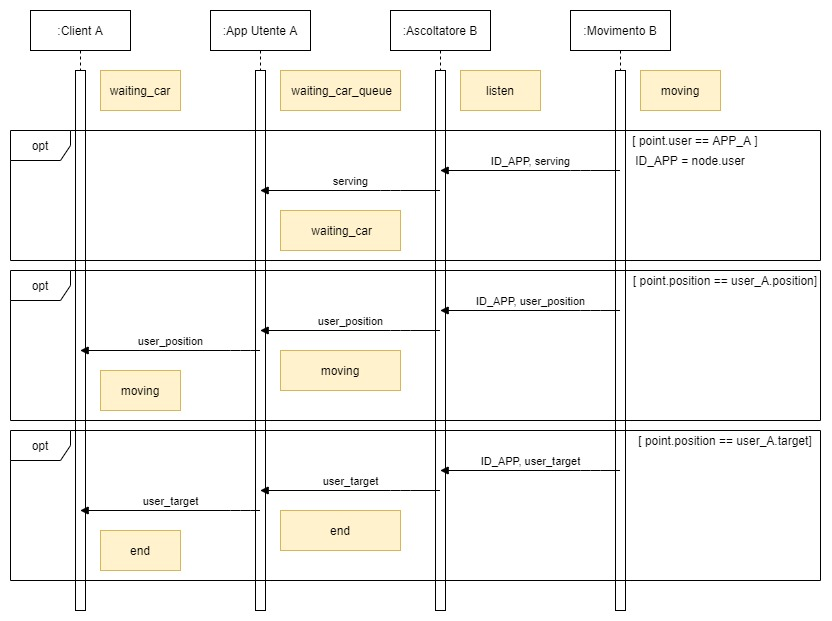
\includegraphics[width=10cm]{messaggi_utente_trasporto.jpg}
	\caption{Messaggi scambiati per il trasporto dell'utente.}
	\label{fig:messaggi_utente_trasporto}
\end{figure}

\begin{figure}[htbp]
	\centering
	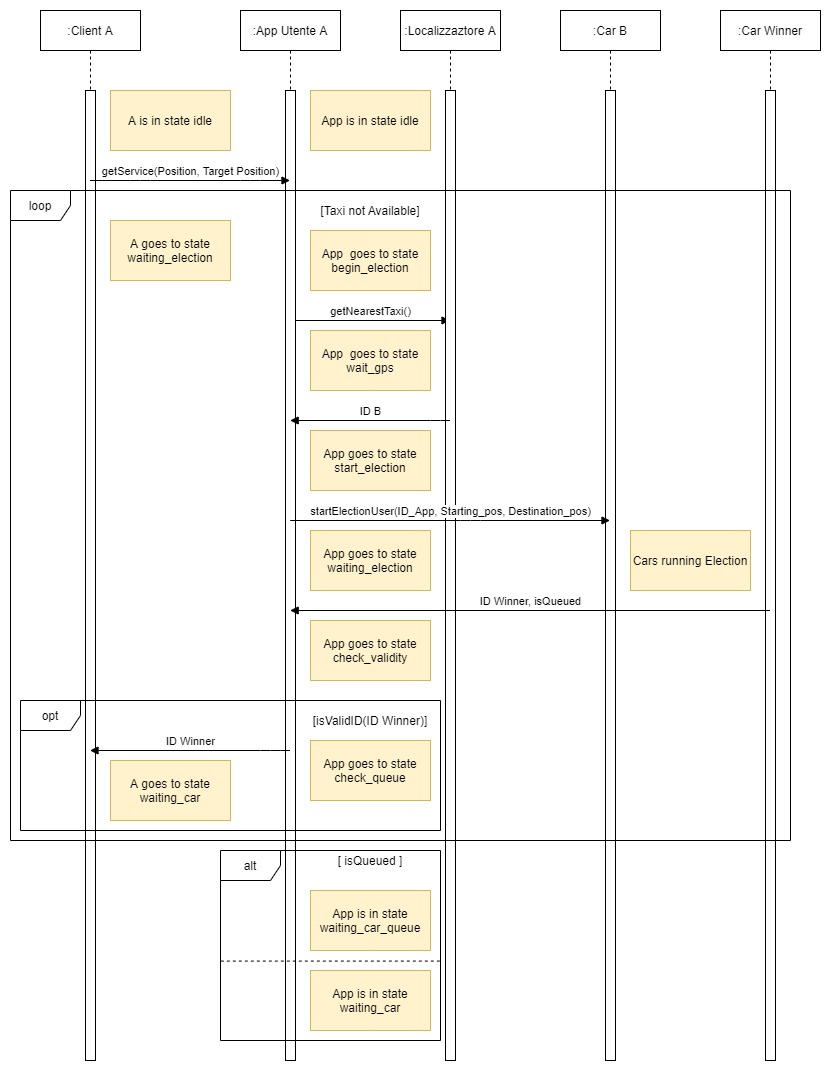
\includegraphics[width=15cm]{messaggi_utente_chiede_macchina.jpg}
	\caption{Messaggi scambiati per la richiesta di un trasporto.}
	\label{fig:messaggi_utente_chiede_macchina}
\end{figure}

\begin{figure}[htbp]
	\centering
	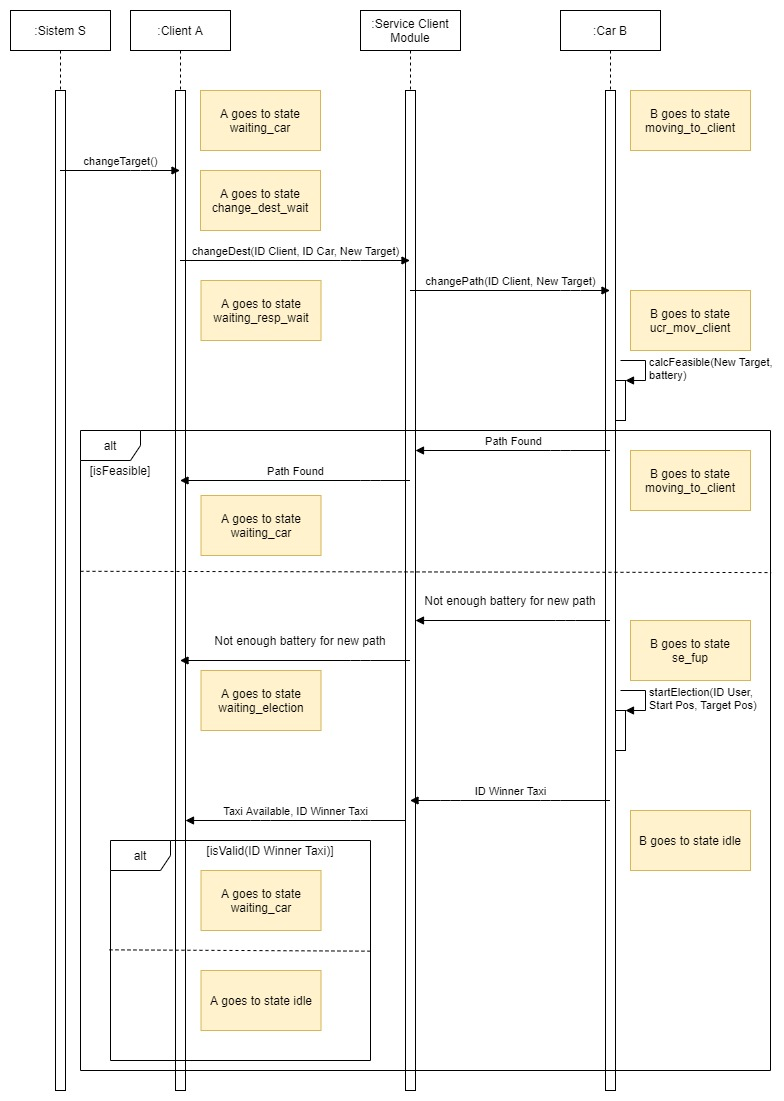
\includegraphics[width=15cm]{messaggi_utente_cambio_direzione_waiting.jpg}
	\caption{Messaggi scambiati per la richiesta di cambiamento di destinazione mentre il taxi è in viaggio verso l'utente.}
	\label{fig:messaggi_utente_cambio_direzione_waiting}
\end{figure}

\begin{figure}[htbp]
	\centering
	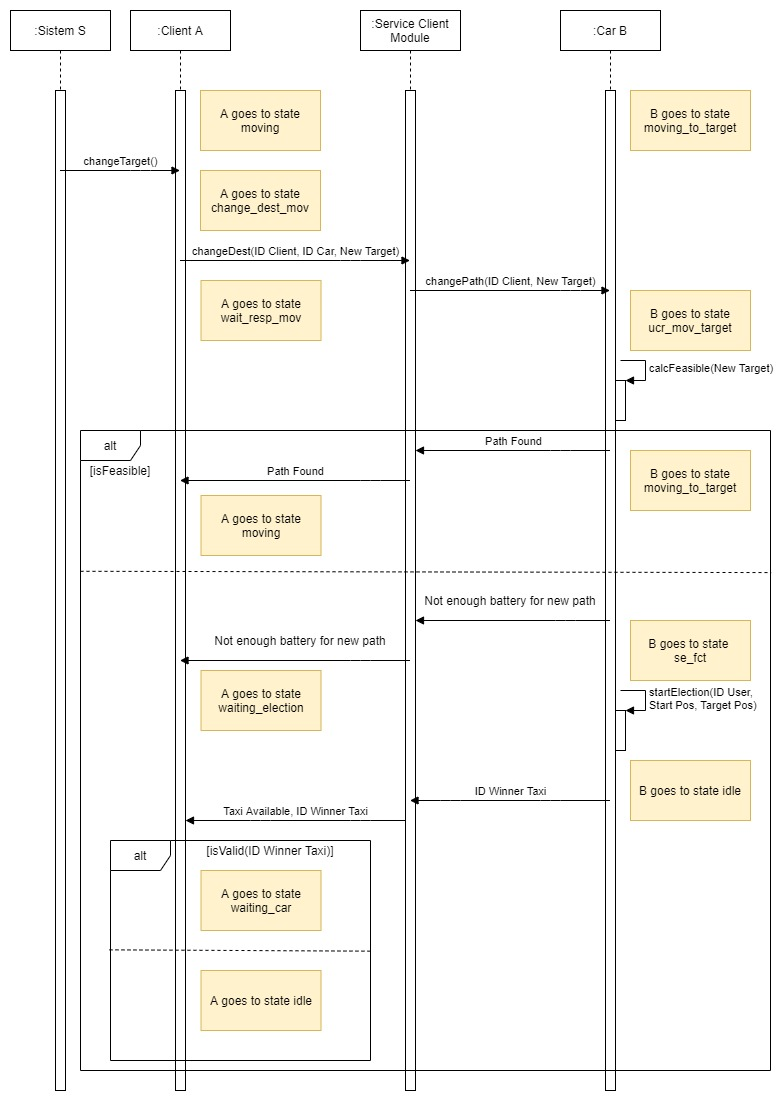
\includegraphics[width=15cm]{messaggi_utente_cambio_direzione_moving.jpg}
	\caption{Messaggi scambiati per la richiesta di cambiamento di destinazione mentre il taxi sta trasportando l'utente.}
	\label{fig:messaggi_utente_cambio_direzione_moving}
\end{figure}

\begin{figure}[htbp]
	\centering
	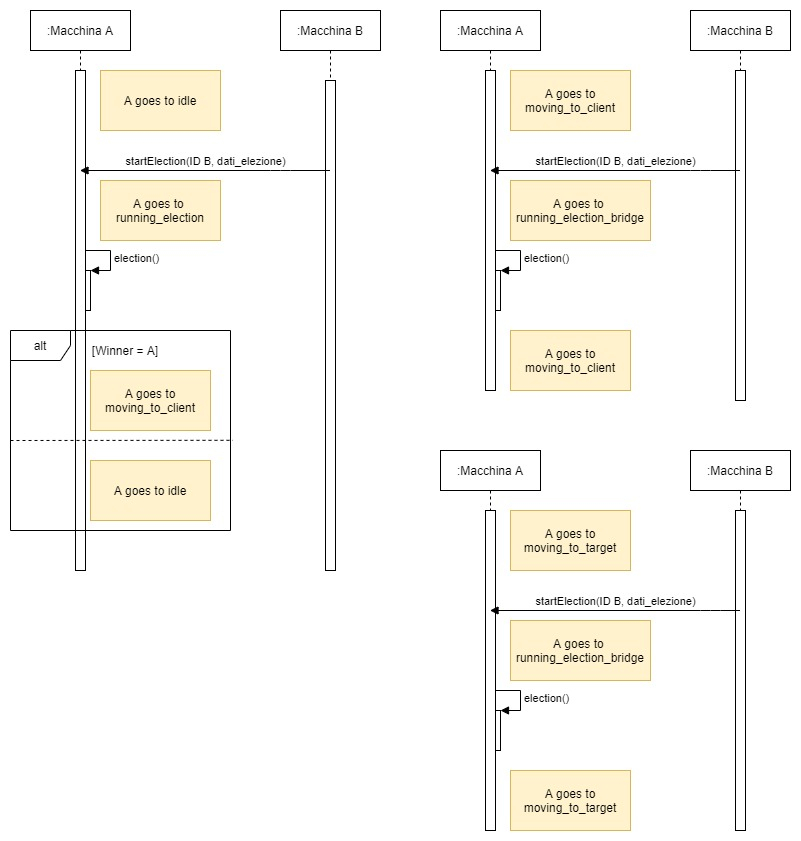
\includegraphics[width=15cm]{messaggi_macchina_partecipazione_elezione.jpg}
	\caption{Partecipazione di una macchina non iniziatrice all'algoritmo dell'elezione.}
	\label{fig:messaggi_macchina_partecipazione_elezione}
\end{figure}

\begin{figure}[htbp]
	\centering
	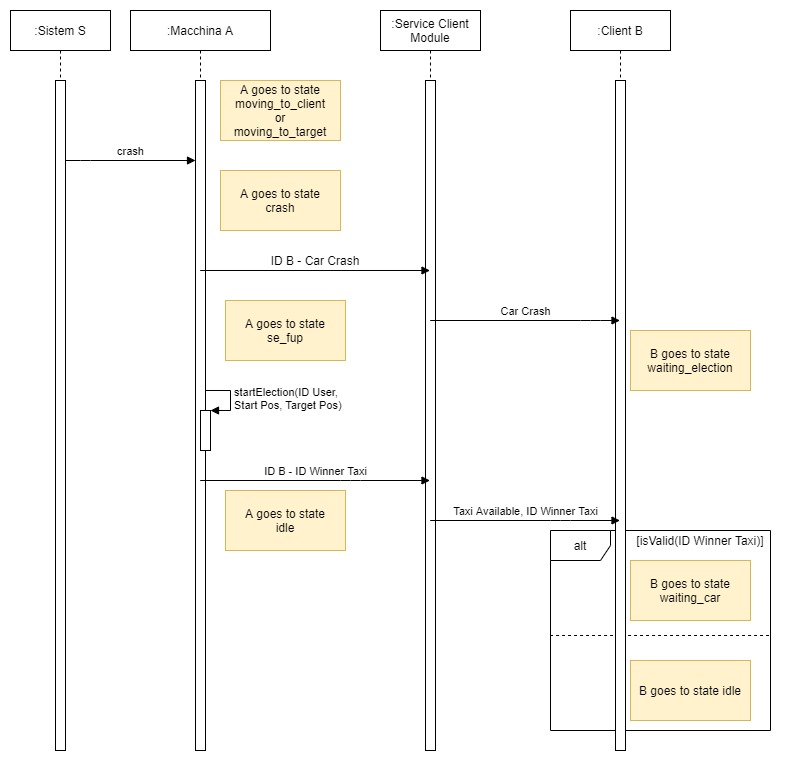
\includegraphics[width=15cm]{messaggi_macchina_crash.jpg}
	\caption{Incidente e notifica all'utente.}
	\label{fig:messaggi_macchina_crash}
\end{figure}

\begin{figure}[htbp]
	\centering
	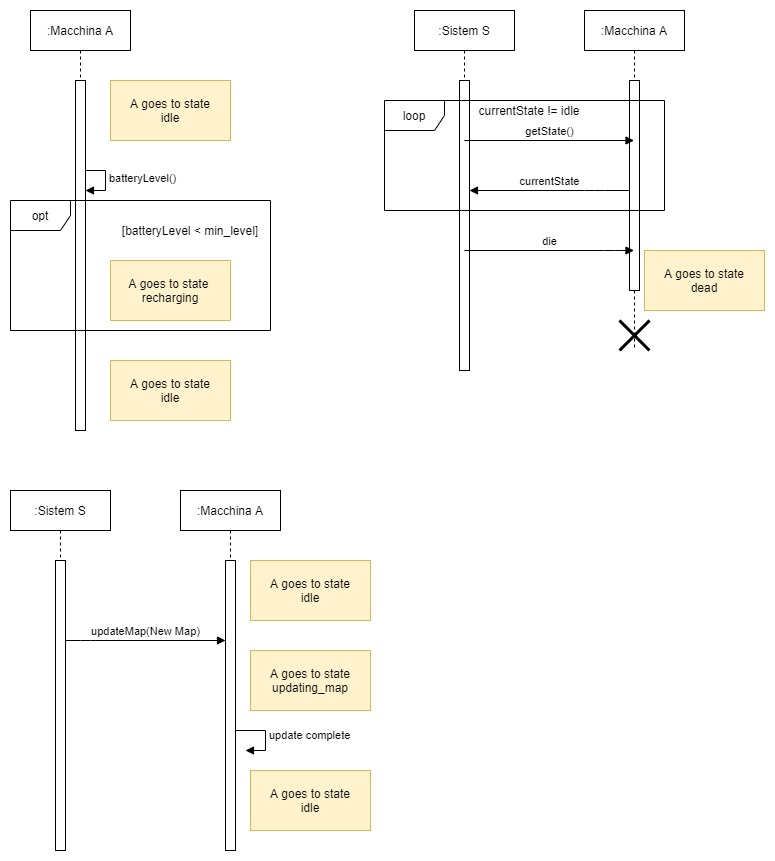
\includegraphics[width=15cm]{messaggi_macchina_batteria_morte_mappaIdle.jpg}
	\caption{Messaggi per la gestione della ricarica, della rimozione e aggiornamento della mappa di un taxi.}
	\label{fig:messaggi_macchina_batteria_morte_mappaIdle}
\end{figure}

\begin{figure}[htbp]
	\centering
	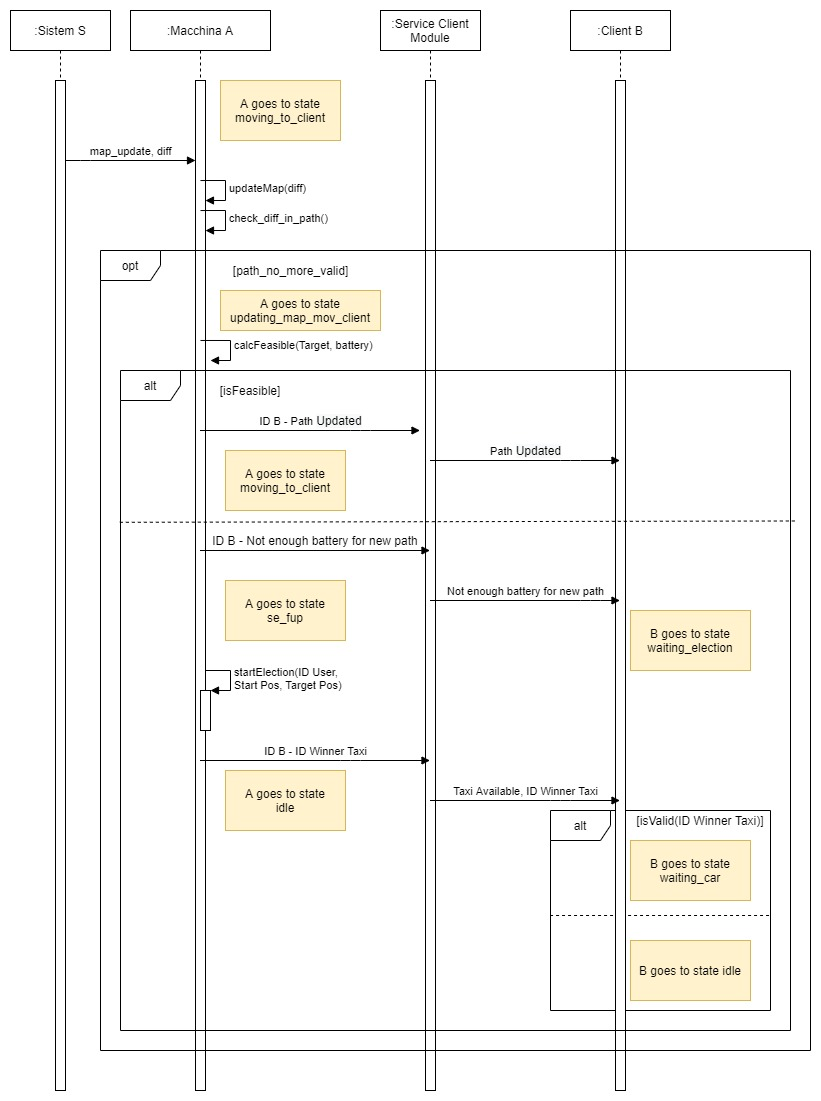
\includegraphics[width=15cm]{messaggi_macchina_aggiornamento_mappa_to_client.jpg}
	\caption{Messaggi per l'aggiornamento della mappa della città mentre il taxi è in viaggio verso un utente.}
	\label{fig:messaggi_macchina_aggiornamento_mappa_to_client}
\end{figure}

\begin{figure}[htbp]
	\centering
	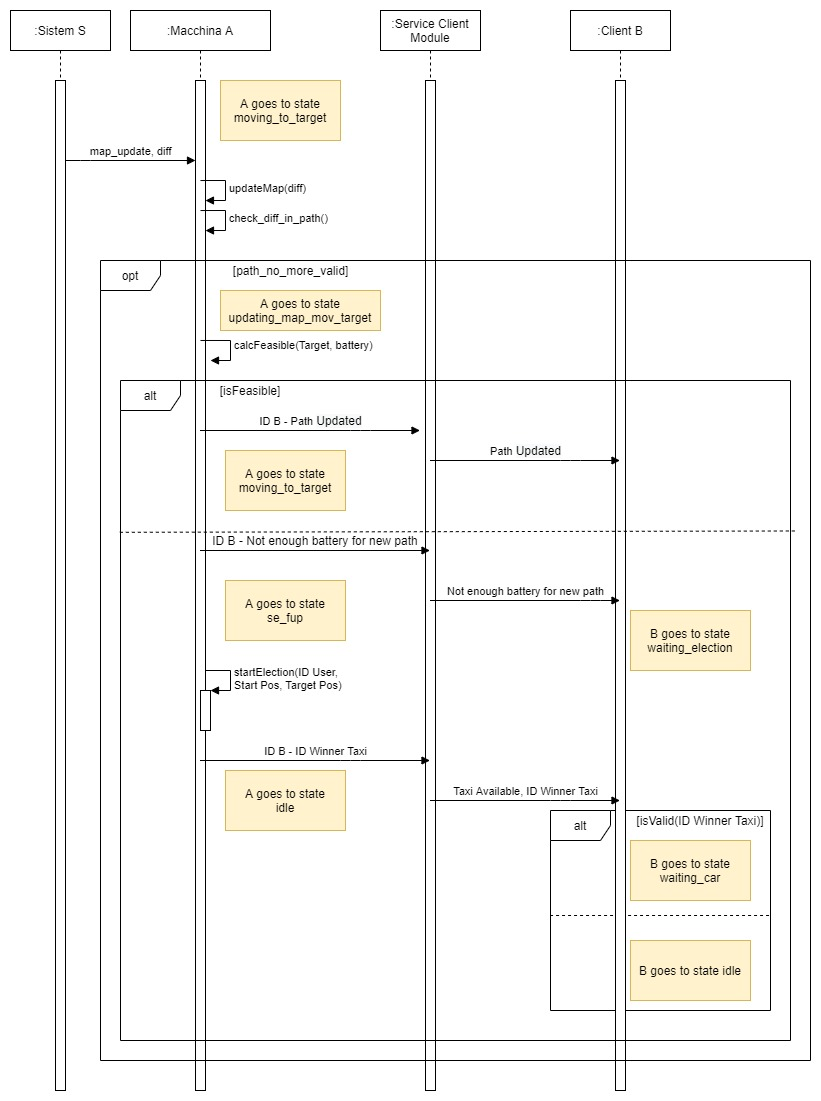
\includegraphics[width=15cm]{messaggi_macchina_aggiornamento_mappa_to_target.jpg}
	\caption{Messaggi per l'aggiornamento della mappa della città mentre il taxi trasporta un utente.}
	\label{fig:messaggi_macchina_aggiornamento_mappa_to_target}
\end{figure}

%!TEX TS-program = pdflatex
%!TEX root =progetto_finale.tex
%!TEX encoding = UTF-8 Unicode
     %%%%%%%%%%%%%%%%%%%%
     %                  %
     %  biblio.tex   %
     %                  %
     %%%%%%%%%%%%%%%%%%%%

\begin{thebibliography}{3}
	\selectlanguage{english}
	\frenchspacing
	
\end{thebibliography}
\selectlanguage{italian}
\nonfrenchspacing

\end{document}